% This file was converted to LaTeX by Writer2LaTeX ver. 1.4
% see http://writer2latex.sourceforge.net for more info
\documentclass{article}
\usepackage[ascii]{inputenc}
\usepackage[T3,T1]{fontenc}
\usepackage[english]{babel}
\usepackage[noenc]{tipa}
\usepackage{tipx}
\usepackage[geometry,weather,misc,clock]{ifsym}
\usepackage{geometry}
\geometry{letterpaper, margin=1in}
\usepackage{pifont}
\usepackage{pdfpages}
\usepackage{eurosym}
\usepackage{amsmath}
\usepackage{multicol}
\usepackage{graphicx}
\graphicspath{ {../jpg/} }
\usepackage{wasysym}
\usepackage{amssymb,amsfonts,textcomp}
\usepackage{array}
\usepackage{supertabular}
\usepackage{hhline}
\usepackage{graphicx}
\makeatletter
\newcommand\arraybslash{\let\\\@arraycr}
\makeatother
\setlength\tabcolsep{1mm}
\renewcommand\arraystretch{1.3}
\title{``This is for young ears'': A Response to Elsa Justel's Marelle...}
\begin{document}

\maketitle

A black box room packed with a rather large audience surrounded by 16 Genelec speakers set as two rings of 8, with an elevation of about 1.5 meters. I arrived just in time for the concert and there were barely any seats left. I sat at the back with my head right behind speaker no. 5 --a quite `bad' location to listen to spatialized music inside a dome. I had the old fear one might encounter in an electroacoustic concert if one is not sitting around the `sweet spot'.\footnote{``From the vantage point of the sweet spot, the listener is not only able to perceive spatial imagery at the loudspeaker locations, but also phantom images in between'' (Kendall, 2010). Based on `precedence' (``the auditory system's mechanism for clarifying directional hearing in reverberant environments''), the size of the area between speakers ``makes a huge difference for listeners outside the sweet spot''. However, he continues, ``signal processing can reshape the situation'' by ``image dispersion'' and ``signal decorrelation''. } Despite my fears --and this is why I am writing this--, Dr. Justel started playing \textit{Marelle}\footnote{\textit{Marelle or the Moments of Life} was premiered on March 29, 2017, \'ElectroBelge, Espace Senghor, Brussels (Belgium) [https://www.electrocd.com/en/oeuvre/42489/Elsa\_Justel/Marelle\_or\_the\_Moments\_of\_Life]. The performance mentioned here happened on June 2017, at NYCEMF} and I could listen to her music inside the entire space in front of me. How did she achieve a complete multidimensional image that can be grasped from a point other than the center of the listening space? To what extent is this composition inherent to a particular spatial distribution? How can I go about showing this? This text is my response to her use of space. 


\begin{flushright}
\textit{
``La rayuela se juega con una piedrita que hay que empujar con la punta del zapato. Ingredientes: una acera, una piedrita, un zapato, y un bello dibujo con tiza, preferentemente de colores. }
\end{flushright}



When Dr. Justel kindly sent me the stems, for the purposes of this response, she explained that the tracks should be assigned in pairs in the space. She emphasized this was of extreme importance since there would be moments in the piece where unwanted gaps in the aural image would emerge should the tracks be assigned in a circular manner. In order to visualize this, I made two puredata (Pd) patches to analyze and plot time-varying spectral images of each track and went ahead and placed them in pairs and in circles. I only show here the paired view.\footnote{The result of assigning a circular count to the track numbers instead of a paired one mostly affects the sides of the aural image. This means that while the front is left unchanged (1-2, 9-10), and the back is swapped (8-7, 16-15), the stereo image of the sides is reconfigured in this way: the right side of the remaining pairs are placed as a stereo image in itself, and the left side of the remaining pairs are placed as another stereo image. This is indeed a very different result in the stereo pairing.}

\begin{center}

En lo alto est\'{a} el Cielo, abajo est\'{a} la Tierra, es muy dif\'{i}cil llegar con la piedrita al Cielo, 

\end{center}

\begin{figure*}
\begin{multicols}{2}
    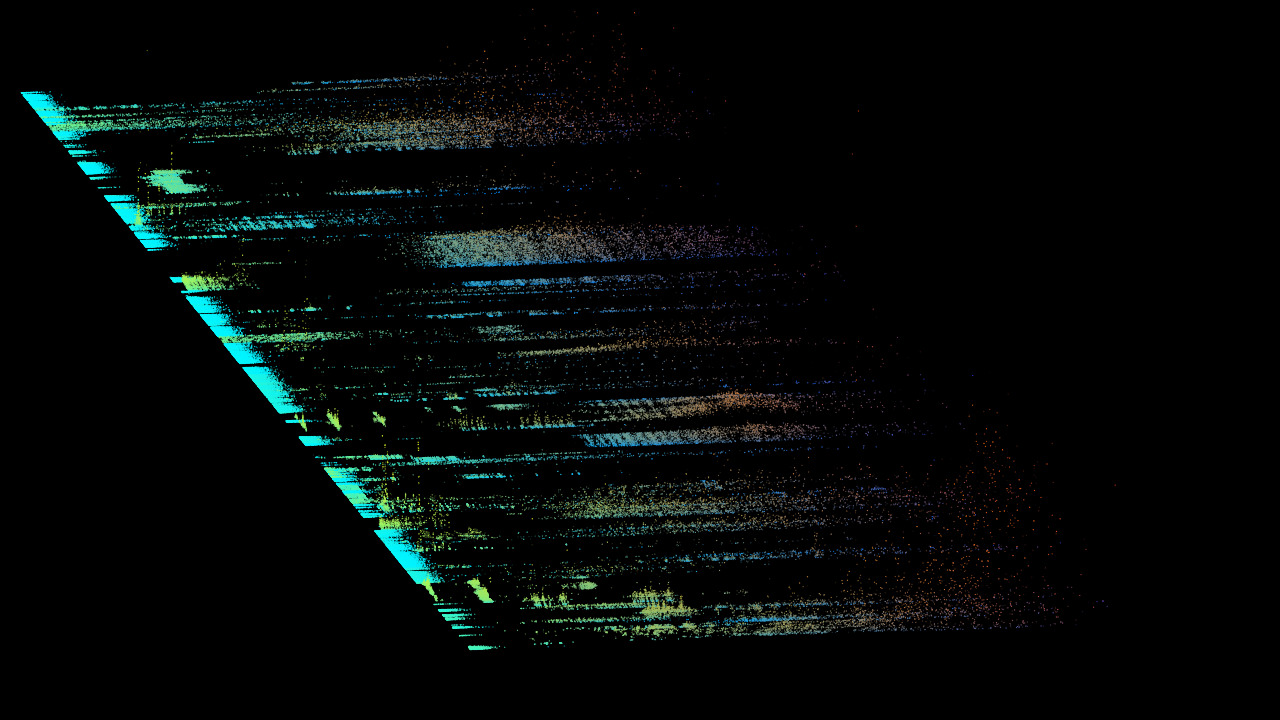
\includegraphics[width=\linewidth]{preset-50-9.jpg}%\par 
    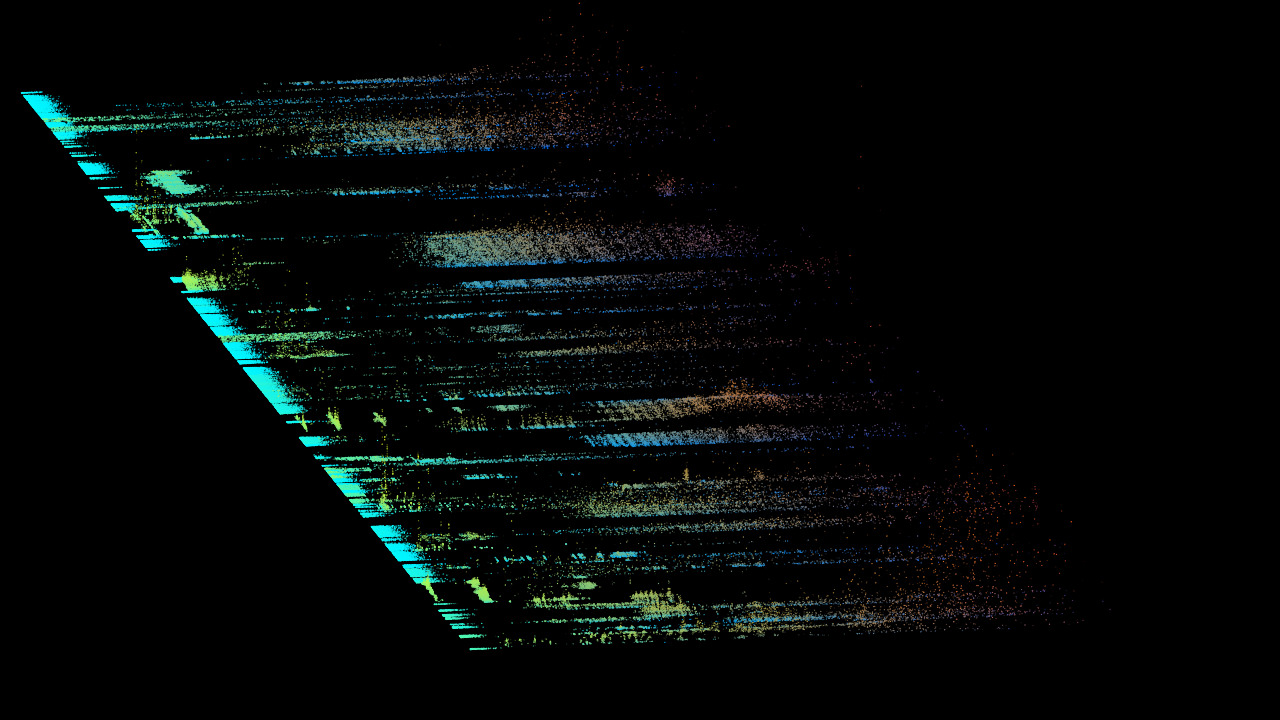
\includegraphics[width=\linewidth]{preset-50-10.jpg}%\par 
    \end{multicols}
\begin{multicols}{2}
    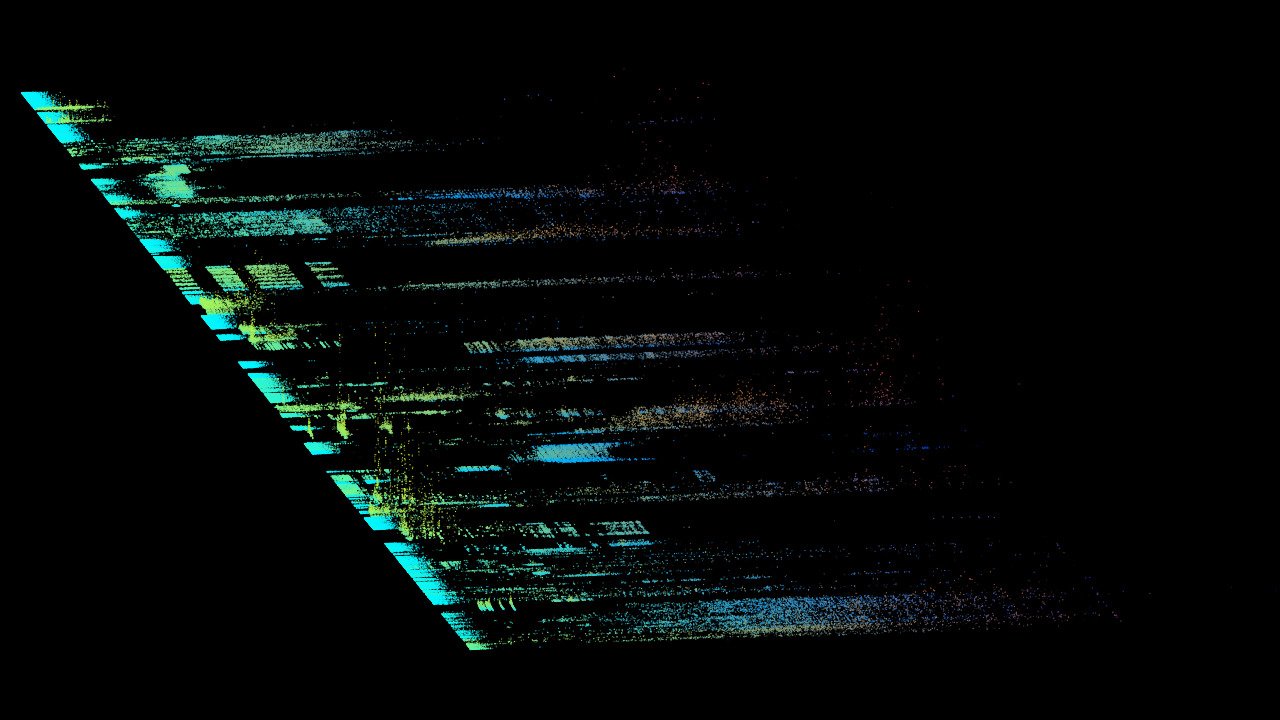
\includegraphics[width=\linewidth]{preset-50-1.jpg}%\par
    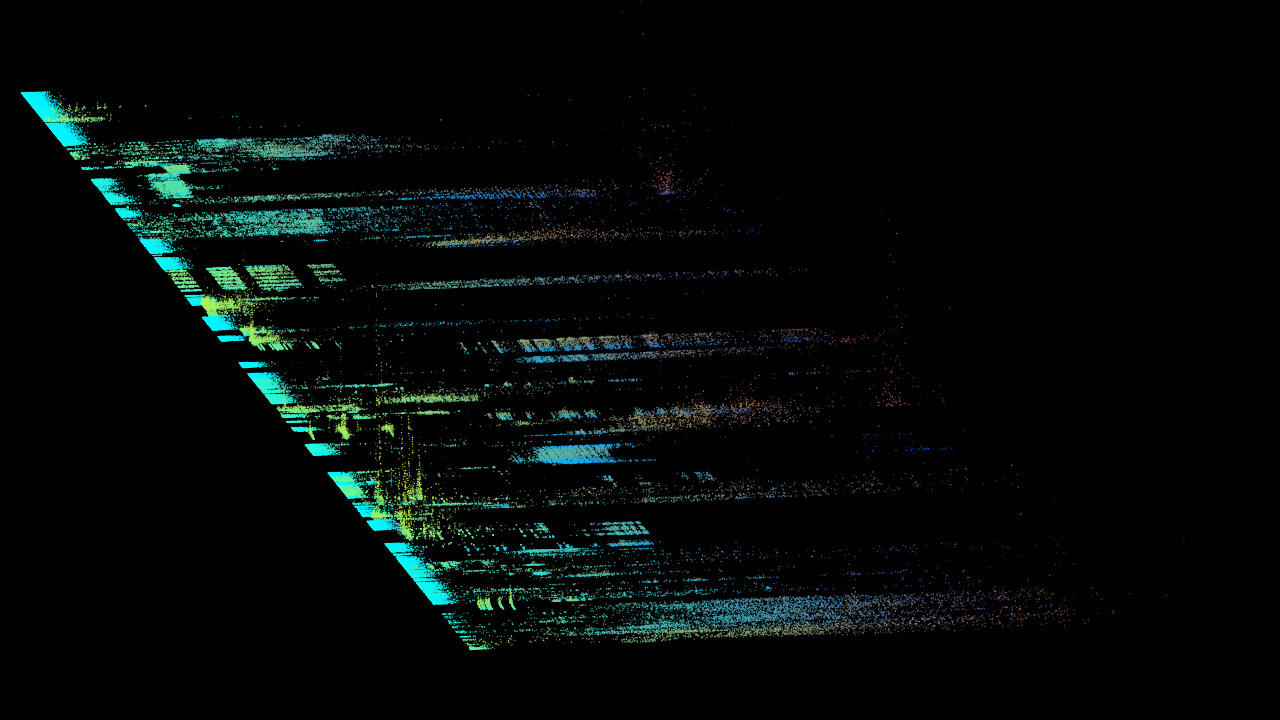
\includegraphics[width=\linewidth]{preset-50-2.jpg}%\par
\end{multicols}
\caption{Tracks 1-2 (below) and 9-10 (above). See Figure 2 for reference.}
\end{figure*}




\newpage

Before going to the visualization, a few things need to be mentioned. I chose puredata's vanilla external [sigmund\~{}] as the workhorse for analysis. Because of this, I ran into several known problems. First of all, the disadvantages regarding the use of Fourier-based spectrum analysis. Particularly in the context of electroacoustic music analysis, ``Fourier analysis is an inherently inefficient way to analyze noisy sounds, since it assumes that these sounds are combinations of harmonically related sinusoids.''\footnote{(Roads, 1996) p.592} Despite these limitations, given that I was given each individual track as rendered by the composer and, more precisely, that these tracks contained mostly synthesized sounds, I considered it to be a very accurate analysis method. Since \textit{Marelle}'s textures are made of very sharp noises subject to highly crafted filtering, a Fourier-based \ \ \ \ \ \ \ \ \ \ \ \ \ \ \ \ \ \ \ \ \ \ \ \ \ \ \ \ \ \ \ \ \ \ \ \ \ \ \ \ \ \ \ \ \ \ \ \ \ \ \ \ \ \ \ \ \ \ \ \ \ \ \ \ \ \ \ \ \ \ \ \ \ \ \ \ \ \ \ \ \ \ \ \ \ \ \ \ \ \ \ \ \ \ \ \ \ \ \ \ \ \ \ \ \ \ \ \ \ \ \ \ \ \ \ \ \ \ \ \ \ \ \ \ \ \ \ \ \ \ \ \ \ \ \ \ \ \ \ \ \ \ \ \ \ \ \ \ \ \ \ \ \ \ \ \ \ \ \ \ \ \ \ \ \ \ \ \ \ \ \ \ \ \ \ \ \ \ \ \ \ \ \ \ \ \ \ \ \ \ \ \ \ \ \ \ \ \ \ \ \ \ \ \ \ \ \ \ \ \ \ \ \ \ \ \ \ \ \ \ \ \ \ \ \ \ \ \ \ \ \ \ \ \ \ \ \ \ \ \ \ \ \ \ \ \ \ \ \ \ \ \ \ \ \ \ \ \ \ \ \ \ \ \ \ \ \ \ \ \ \ \ \ \ \ \ \ \ \ \ \ \ \ \ \ \ \ \ \ \ \ \ \ \ \ \ \ \ \ \ \ \ \ \ \ \ \ \ spectral


\bigskip

\begin{center}
\textit{casi siempre se calcula mal y la piedra sale del dibujo. }

\end{center}

\bigskip

\ \ \ \ \ \ \ \ \ \ \ \ \ \ \ \ \ \ \ \ \ \ \ \ \ \ \ \ \ \ \ \ \ \ \ \ \ \ \ \ \ \ \ \ \ \ \ \ \ \ \ \ \ \ \ \ \ \ \ \ \ \ \ \ \ \ \ \ \ \ \ \ \ \ \ \ \ \ \ \ \ \ \ \ \ \ \ \ \ \ \ \ \ \ \ \ \ \ \ peak \ \ \ \ \ \ \ \ \ \ \ \ \ \ \ analysis would detect not the noise, but the filtering, giving a rather accurate depiction of the spectral content of the actual sound. Moreover, since these short grains of filtered noise are burst expressively to space and diffused in divergent ways, I would be able to extract motion from one plot to the next if the peaks match in position. I will elaborate on this problem later on.


\bigskip

\begin{flushleft}
Poco a poco, sin embargo, se va adquiriendo la habilidad necesaria para salvar las diferentes casillas (rayuela caracol, rayuela rectangular, rayuela de fantas\'{i}a, poco usada) y un d\'{i}a se aprende a salir de la Tierra y remontar la piedrita hasta el Cielo, 

\end{flushleft}

\newpage

\begin{flushright}
A second drawback of the Fourier based method is known as the ``tradeoff between the number of frequency bins and the length of the analysis window''\footnote{(Roads, 1996) p.559}. In general, what is recommended is to tailor the analysis method to the input source. I have found therefore that a window size of 2048 samples, given the sample rate of 48kHz worked very well to obtain as much frequency resolution as possible. The narrower the window size, the less bins it can resolve and therefore the more accurate frequency distinction it makes. For a sample rate of 48kHz and a total length of 12 minutes (about 3.456e+07 samples per track) the \textbf{Time|Frequency Tradeoffs} table shows results for each of the tracks.

\end{flushright}


\begin{figure*}

\begin{multicols}{2}
    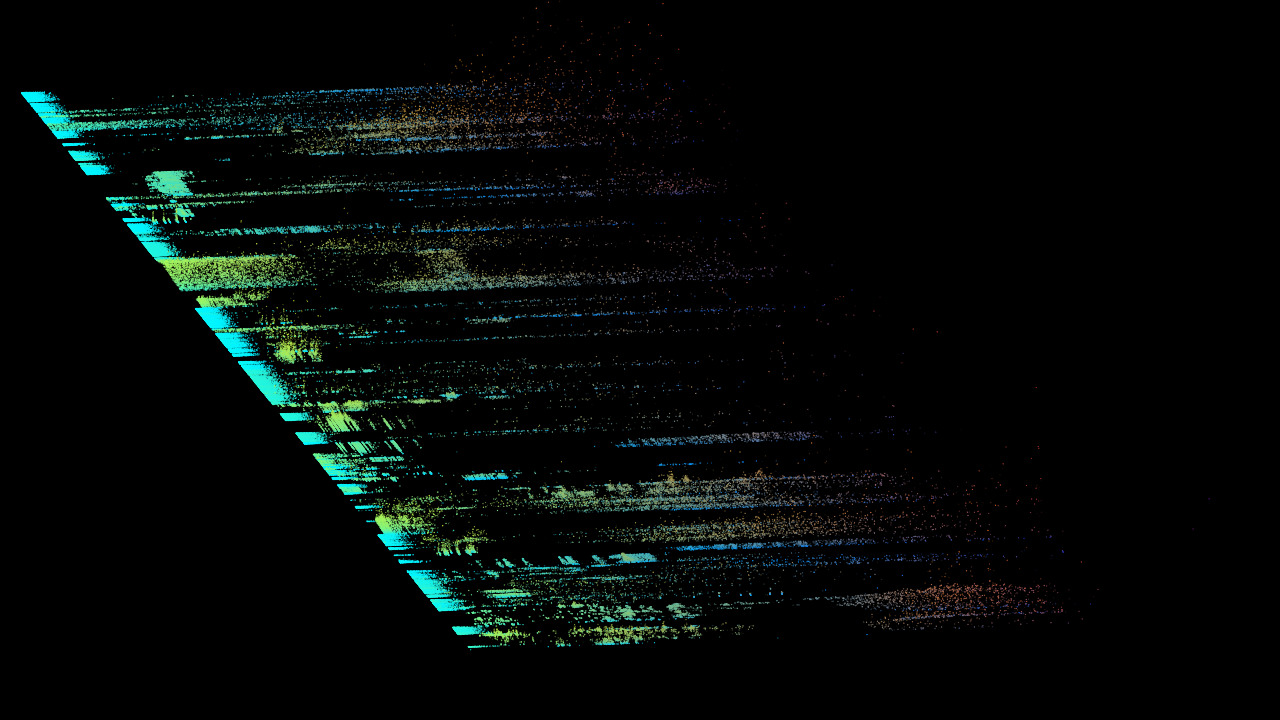
\includegraphics[width=\linewidth]{preset-50-11.jpg}%\par
    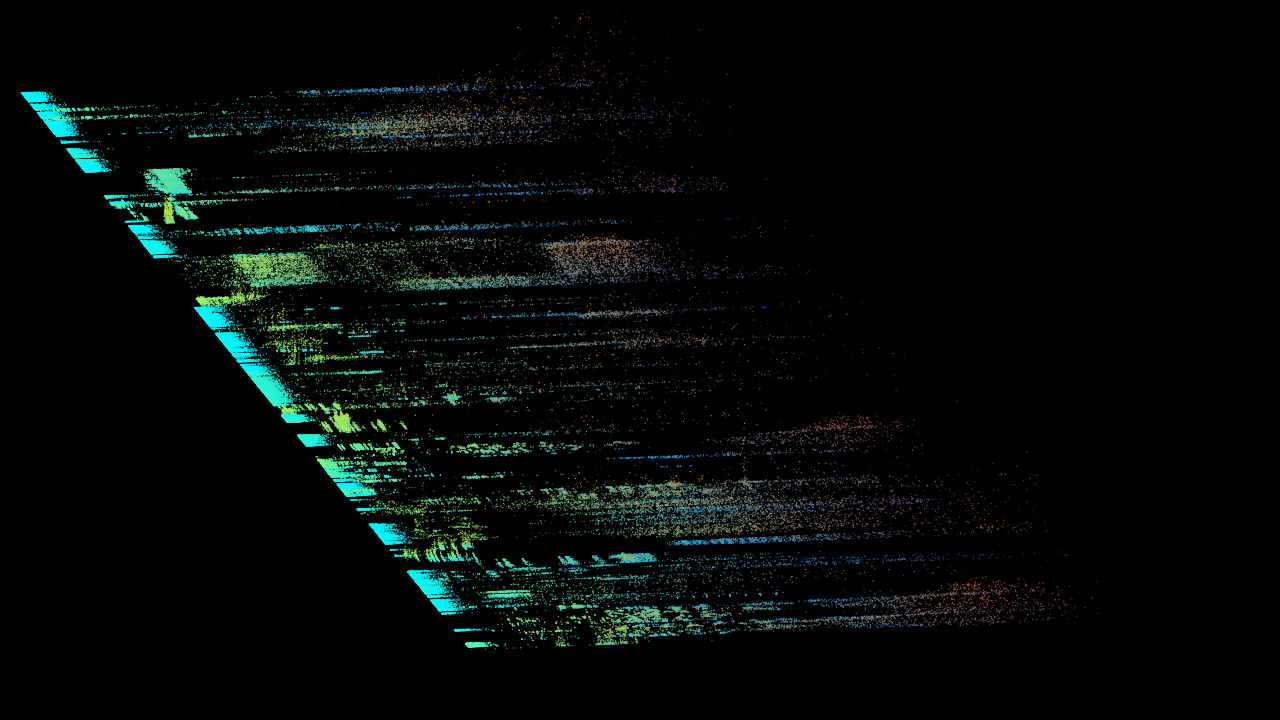
\includegraphics[width=\linewidth]{preset-50-12.jpg}%\par
\end{multicols}

\begin{multicols}{2}
    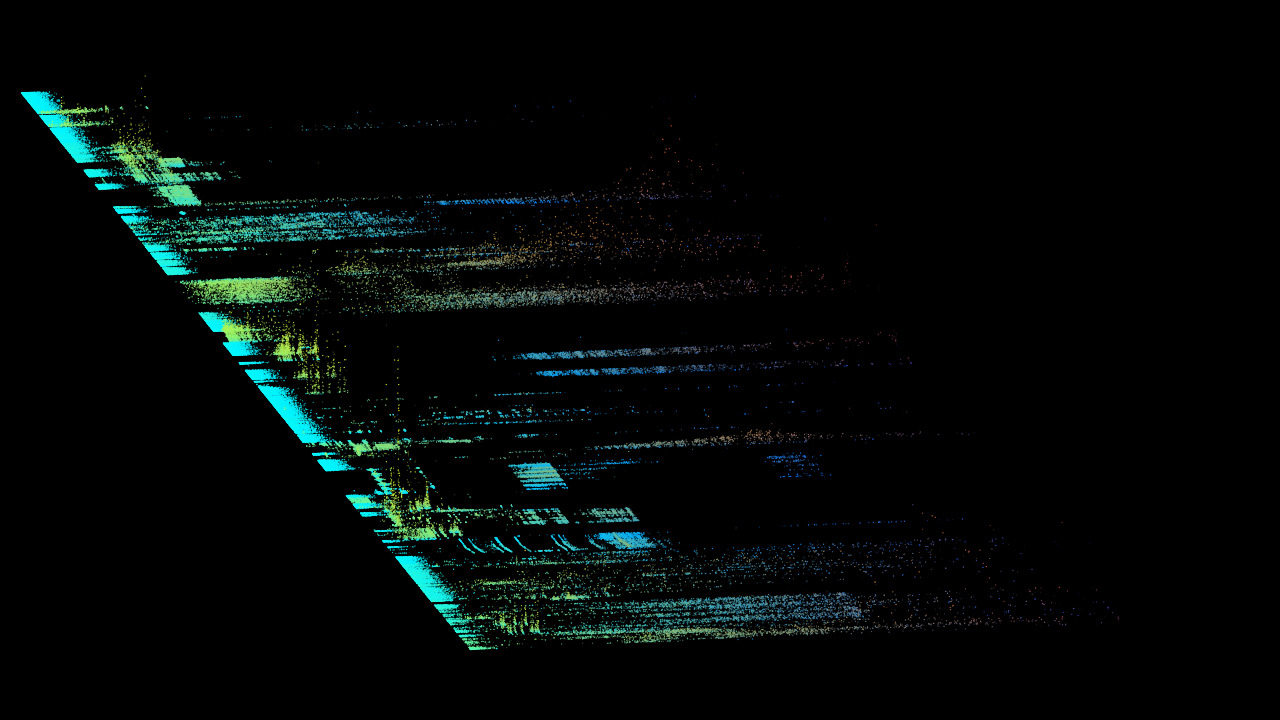
\includegraphics[width=\linewidth]{preset-50-3.jpg}%\par 
    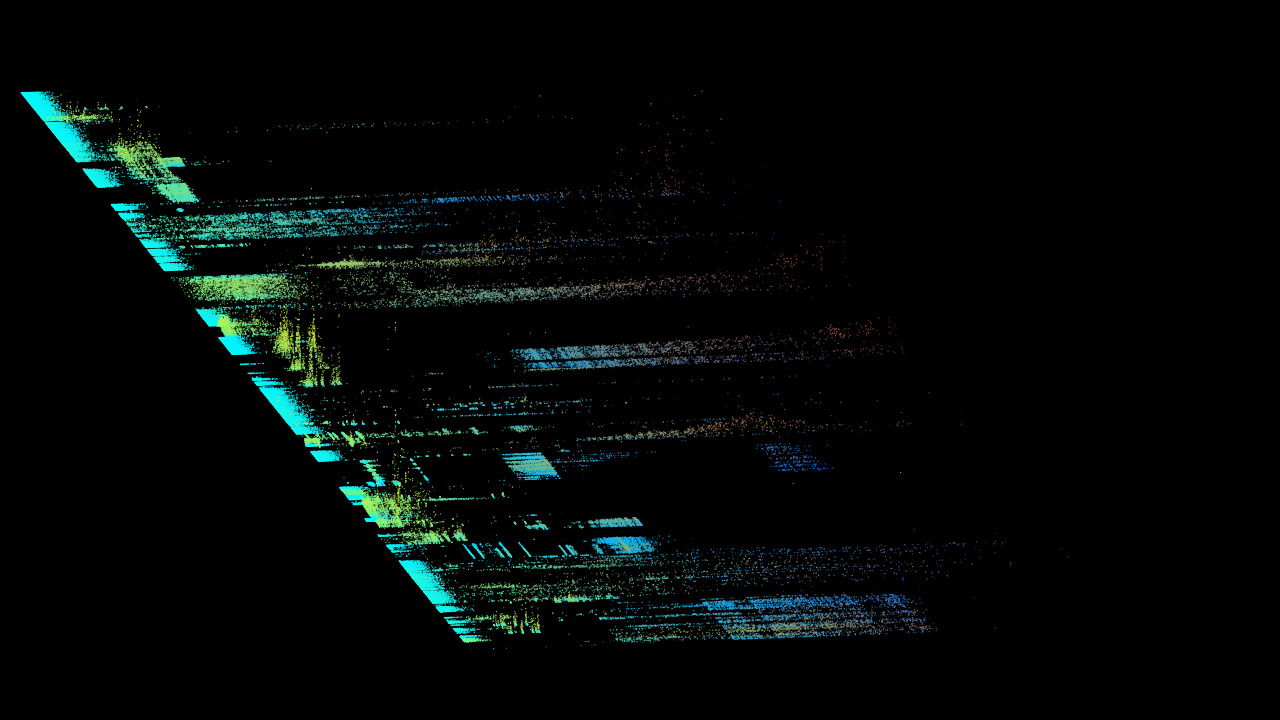
\includegraphics[width=\linewidth]{preset-50-4.jpg}%\par 
\end{multicols}
    
\caption{Tracks 3-4 (below) and 11-12 (above). Frequency is in the X-axis, the leftmost being the highest frequencies (around 16 kHz); Amplitude is in the Y axis, scaled to show the loudest peaks as upward saliences; and Time is in the Z axis from back to front, showing a total duration of 12 minutes.}
\end{figure*}


Finally, the major drawback in using [sigmund\~{}] comes from a rather ambitious need. Since there are 16 different tracks, and since [sigmund\~{}] only outputs peaks if it detected them, then there are variable numbers of peaks in each track. This is what explains the averaging of peak count in the \textbf{Time|Frequency Tradeoffs} table. Because of this decorrelation of peak detection, an analysis of the peaks should be tracked in space. [sigmund\~{}] already has a tracks mode, which performs sequential peak tracking. However, there is not such a tool for spatial tracking. Moreover, there is a dimensional limitation since Pd has only one-dimensional FFT built-in capability.\footnote{Although Pd can host both FFTW and Takuya OOURA's FFT implementation, [simgund\~{}] can only be used with the latter. Moreover, in both these FFT routines a one-dimentional implementation is made in Pd, which is, of course, reasonably enough computation for a large number of audio processing techniques.} 


\begin{figure*}
\begin{center}
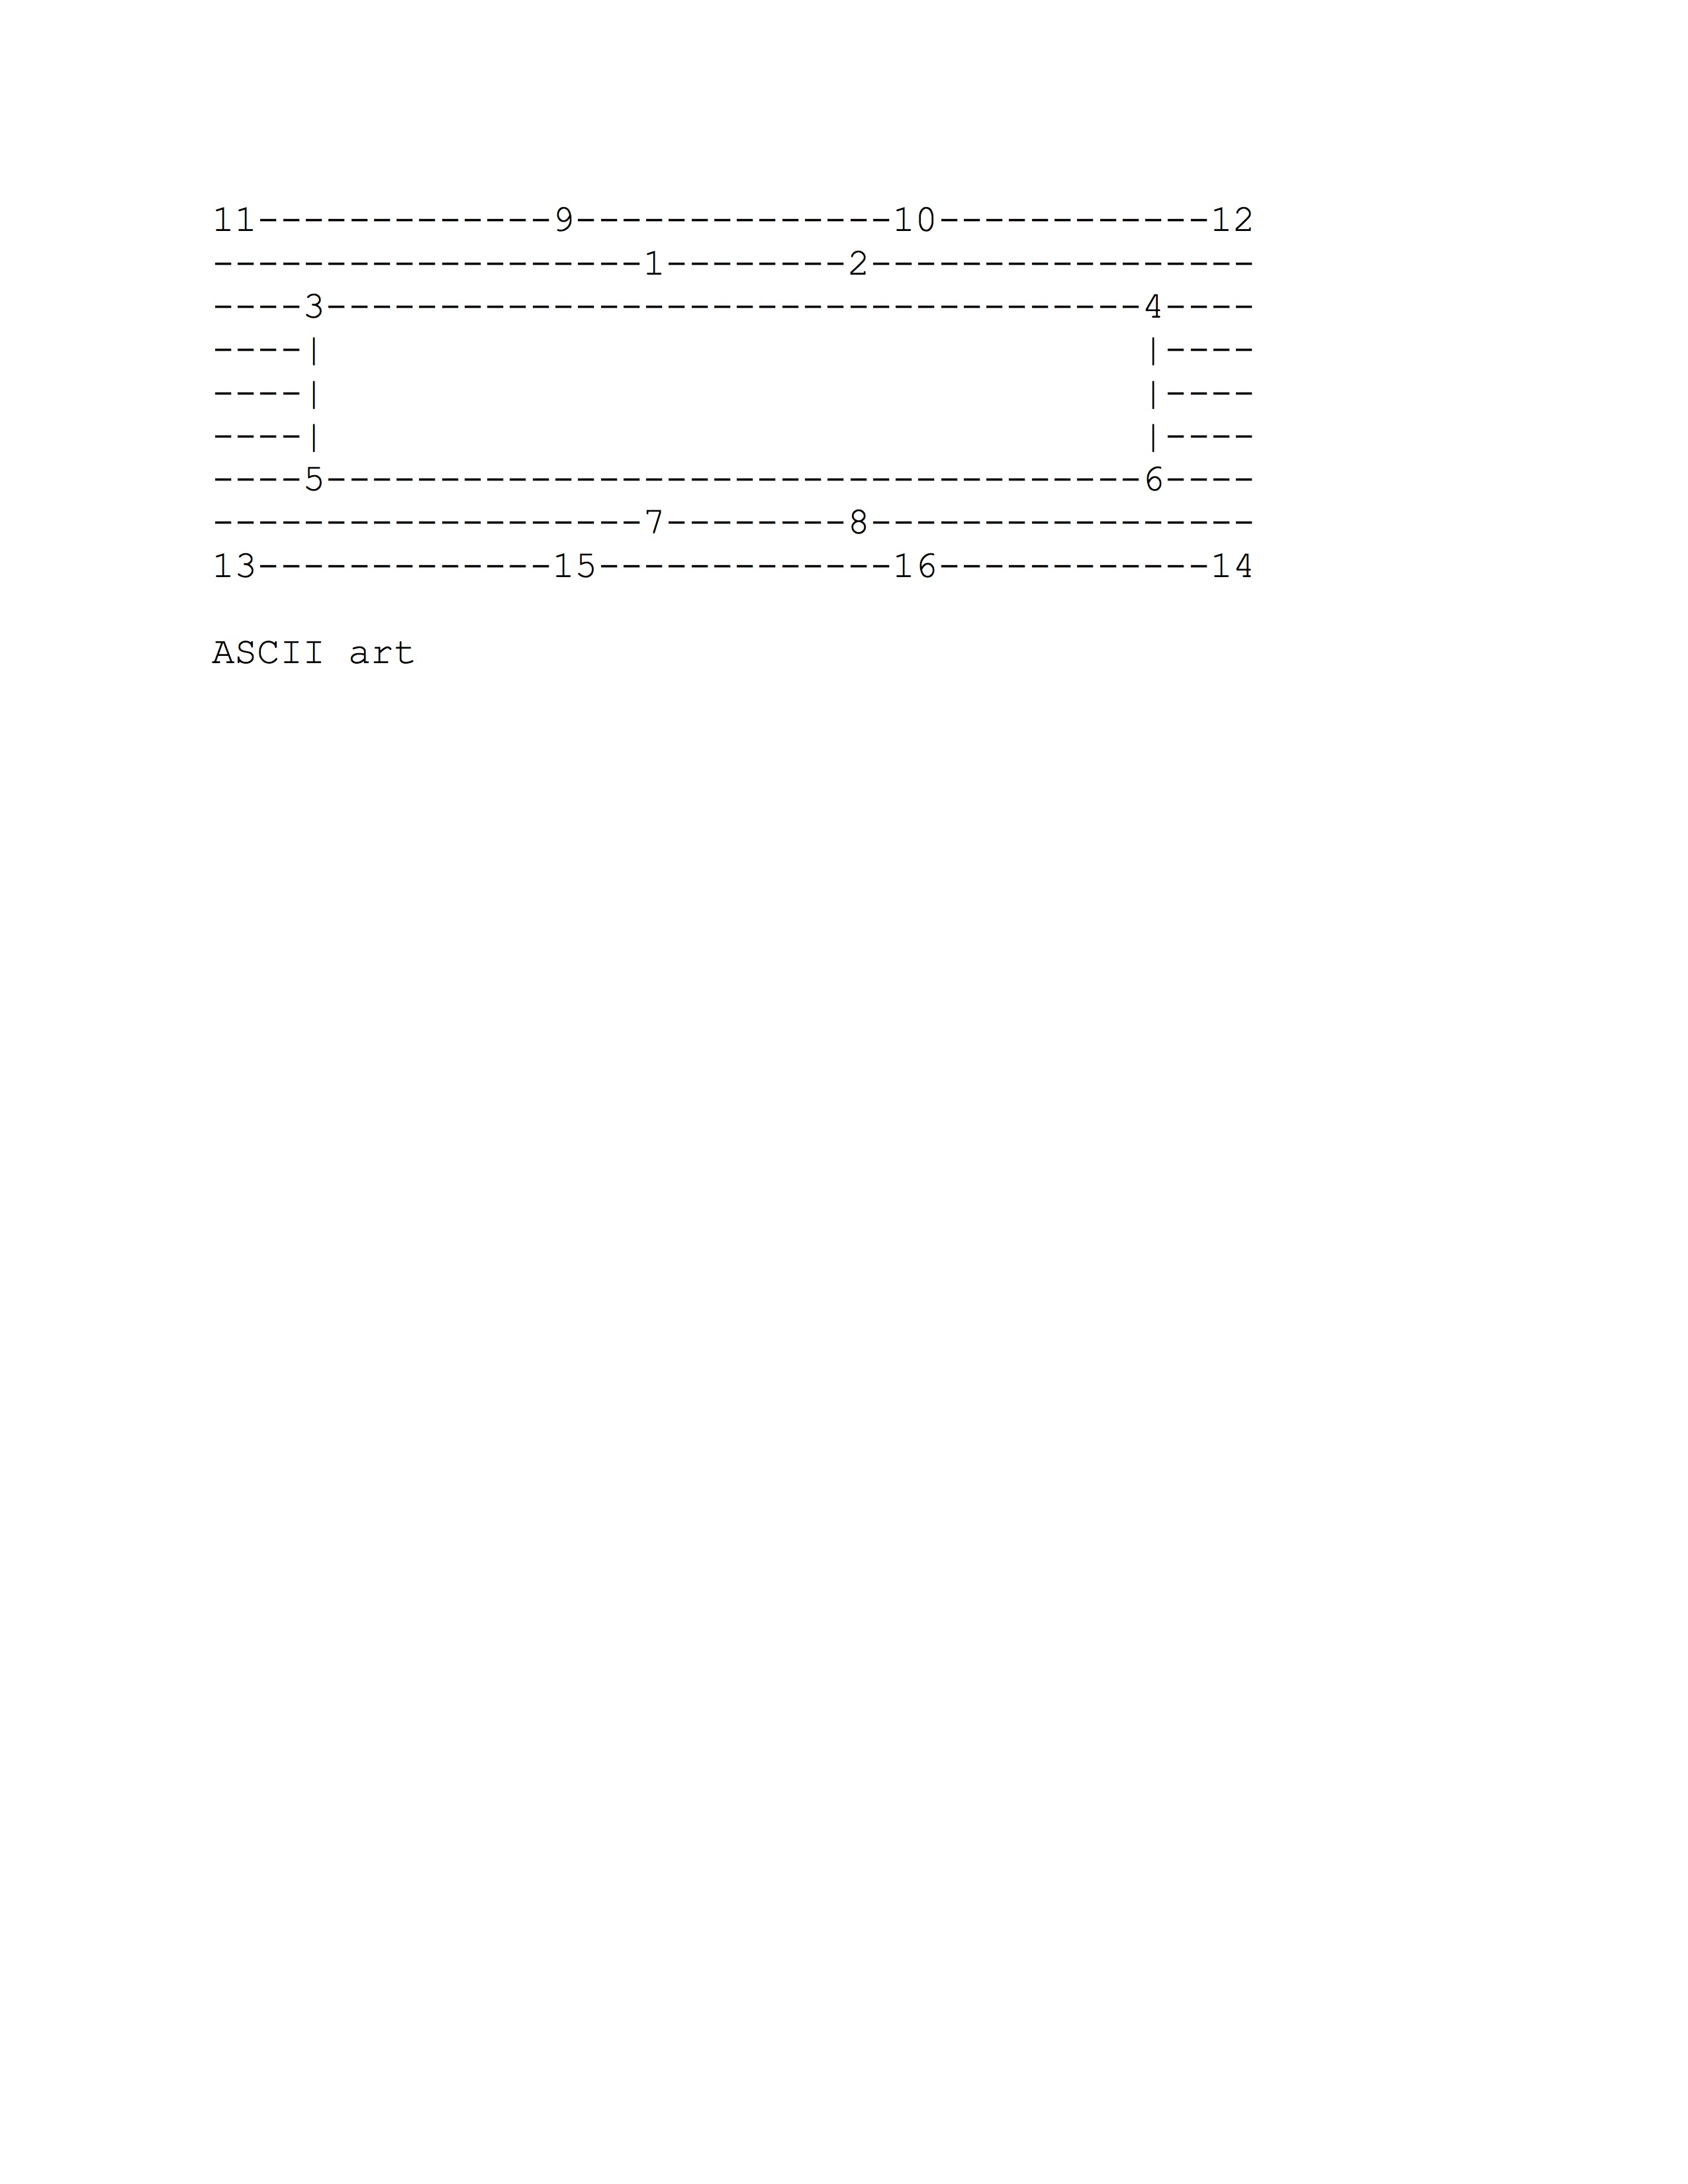
\includegraphics[width=1.5in]{speaker-positions.jpg}
\end{center}
\caption{Speaker Positions}
\end{figure*}




\begin{center}
\textit{Taking a step further, this means that if one is tempted to compute a complete spectral image of the listening space using N tracks, how would a N-dimensional FFT affect multichannel electroacoustic analysis? This question clearly goes beyond the limit of this paper, but it would make an interesting follow-up research.}

\end{center}

\newpage

\begin{flushleft}

\tablefirsthead{}
\tablehead{}
\tabletail{}
\tablelasttail{}
\bottomcaption{Time|Frequency Tradeoffs. This table shows the result of four analysis performed for all tracks in different window sizes. For all these analysis the peak maximum is the same (10) and the "Peak Convergence" (the difference between the targetted peaks and the actual peak average) is shown as a function of the window size. Surprisingly, the greatest margin falls into a window size of 8192, not 16384, and the least margen belonged to a size of 1024. The chosen window size was ultimately 2048, as a compromise between performance and peak convergence.}
\begin{supertabular}{|m{1.4108598in}|m{0.9420598in}|m{0.9837598in}|m{1.0566599in}|m{1.0775598in}|}
\hline
Sample Length &
\raggedleft 3.46E+07 &
\raggedleft 3.46E+07 &
\raggedleft 3.46E+07 &
\raggedleft\arraybslash 3.46E+07\\\hline
Window Size &
\raggedleft 16384 &
\raggedleft 8192 &
\raggedleft 2048 &
\raggedleft\arraybslash 1024\\\hline
Peak Count &
\raggedleft 2130 &
\raggedleft 4720 &
\raggedleft 17118 &
\raggedleft\arraybslash 34238\\\hline
Peak Max &
\raggedleft 10 &
\raggedleft 10 &
\raggedleft 10 &
\raggedleft\arraybslash 10\\\hline
Target Peaks &
\raggedleft 21300 &
\raggedleft 47200 &
\raggedleft 171180 &
\raggedleft\arraybslash 342380\\\hline
Peaks/track no.1 &
\raggedleft 21730 &
\raggedleft 43482 &
\raggedleft 173363 &
\raggedleft\arraybslash 346730\\\hline
Peaks/track no.2 &
\raggedleft 21762 &
\raggedleft 43555 &
\raggedleft 173704 &
\raggedleft\arraybslash 347395\\\hline
Peaks/track no.3 &
\raggedleft 21142 &
\raggedleft 42281 &
\raggedleft 169021 &
\raggedleft\arraybslash 337857\\\hline
Peaks/track no.4 &
\raggedleft 21364 &
\raggedleft 42714 &
\raggedleft 170685 &
\raggedleft\arraybslash 341172\\\hline
Peaks/track no.5 &
\raggedleft 21740 &
\raggedleft 43400 &
\raggedleft 173337 &
\raggedleft\arraybslash 346835\\\hline
Peaks/track no.6 &
\raggedleft 21714 &
\raggedleft 43421 &
\raggedleft 173539 &
\raggedleft\arraybslash 347095\\\hline
Peaks/track no.7 &
\raggedleft 21808 &
\raggedleft 43533 &
\raggedleft 173879 &
\raggedleft\arraybslash 347725\\\hline
Peaks/track no.8 &
\raggedleft 21715 &
\raggedleft 43402 &
\raggedleft 173135 &
\raggedleft\arraybslash 346120\\\hline
Peaks/track no.9 &
\raggedleft 22469 &
\raggedleft 44919 &
\raggedleft 179492 &
\raggedleft\arraybslash 358835\\\hline
\multicolumn{5}{|m{5.7858596in}|}{hasta entrar en el Cielo (Et tous nos amours, solloz\'{o} Emmanu\`{e}le boca abajo),}\\\hline
Peaks/track no.10 &
\raggedleft 22452 &
\raggedleft 44850 &
\raggedleft 179007 &
\raggedleft\arraybslash 357987\\\hline
Peaks/track no.11 &
\raggedleft 22187 &
\raggedleft 44360 &
\raggedleft 176908 &
\raggedleft\arraybslash 353725\\\hline
Peaks/track no.12 &
\raggedleft 22030 &
\raggedleft 43902 &
\raggedleft 174795 &
\raggedleft\arraybslash 349825\\\hline
Peaks/track no.13 &
\raggedleft 22204 &
\raggedleft 44332 &
\raggedleft 177080 &
\raggedleft\arraybslash 354077\\\hline
Peaks/track no.14 &
\raggedleft 21887 &
\raggedleft 43692 &
\raggedleft 174538 &
\raggedleft\arraybslash 349070\\\hline
Peaks/track no.15 &
\raggedleft 22052 &
\raggedleft 44012 &
\raggedleft 175790 &
\raggedleft\arraybslash 351362\\\hline
Peaks/track no.16 &
\raggedleft 22343 &
\raggedleft 44718 &
\raggedleft 178685 &
\raggedleft\arraybslash 357167\\\hline
Average Peaks &
\raggedleft 21912.4375 &
\raggedleft 43785.8125 &
\raggedleft 174809.875 &
\raggedleft\arraybslash 349561.0625\\\hline
Peak Convergence &
\raggedleft 0.9720506904 &
\raggedleft 1.077974744 &
\raggedleft 0.9792352978 &
\raggedleft\arraybslash 0.9794569153\\\hline
\end{supertabular}
\end{flushleft}


\newpage

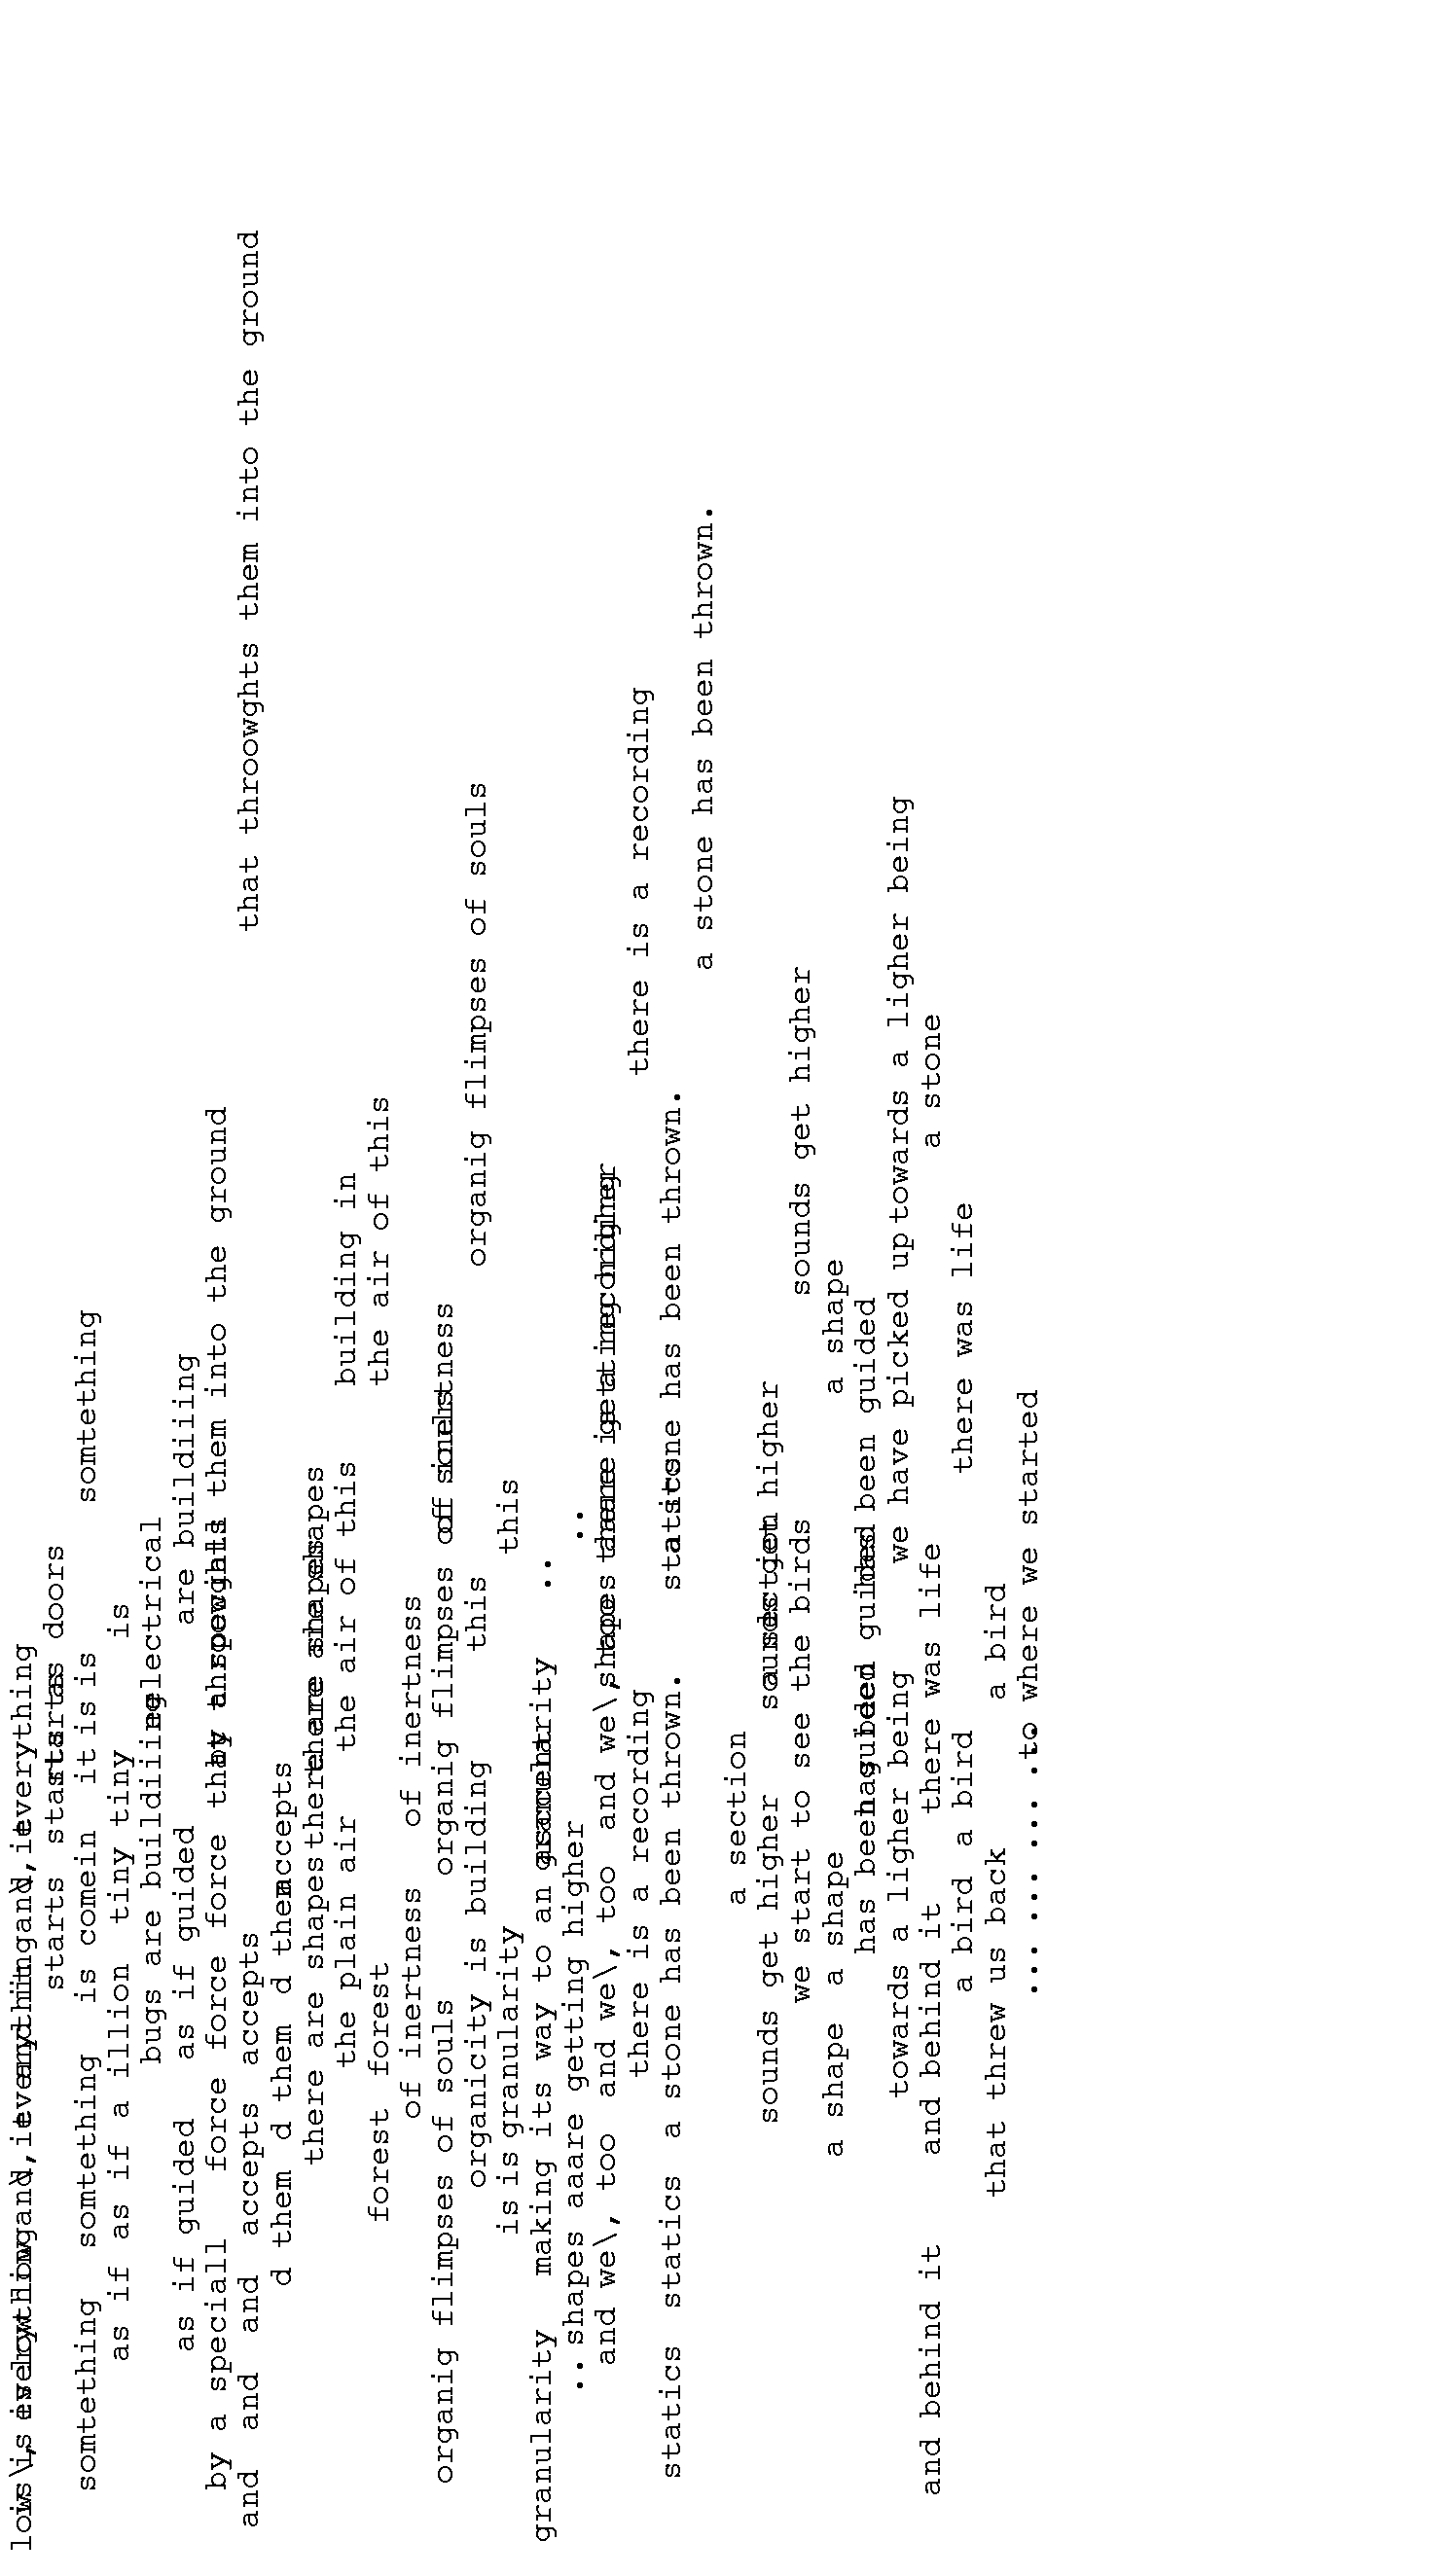
\includepdf[pages={1}]{../pdf/sub-5.pdf}




\begin{figure*}

\begin{multicols}{2}
    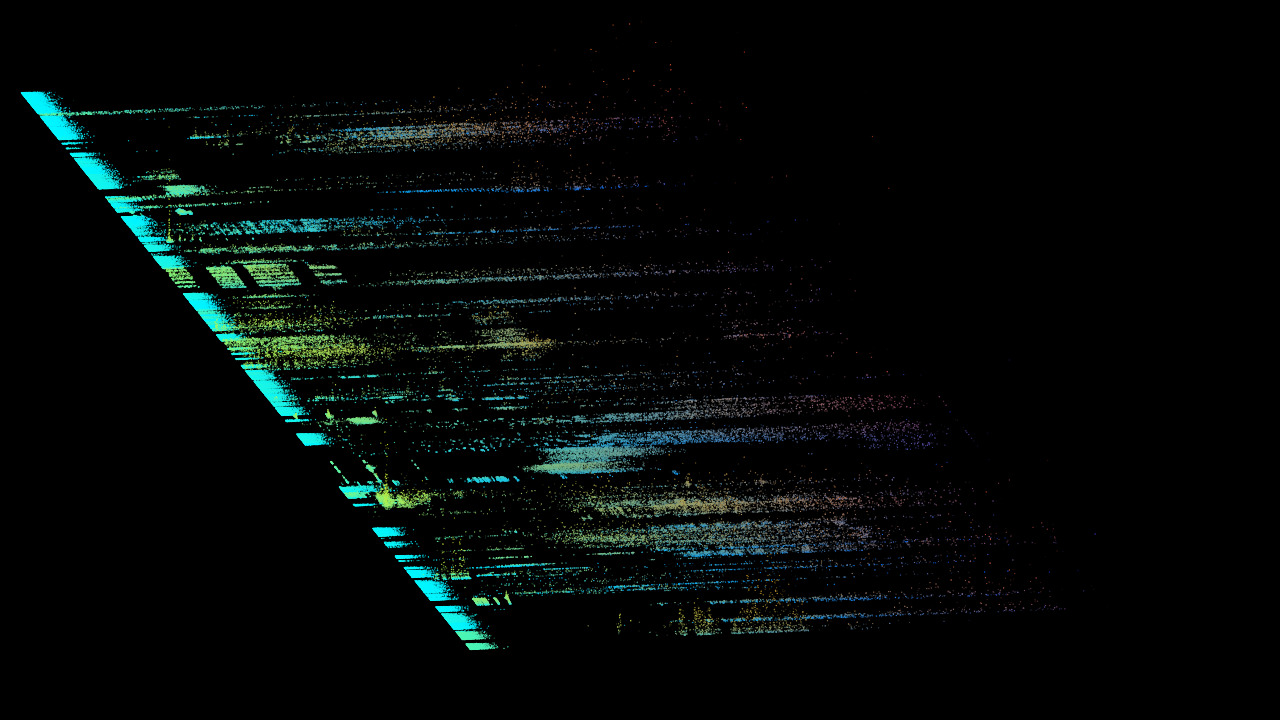
\includegraphics[width=\linewidth]{preset-50-13.jpg}%\par
    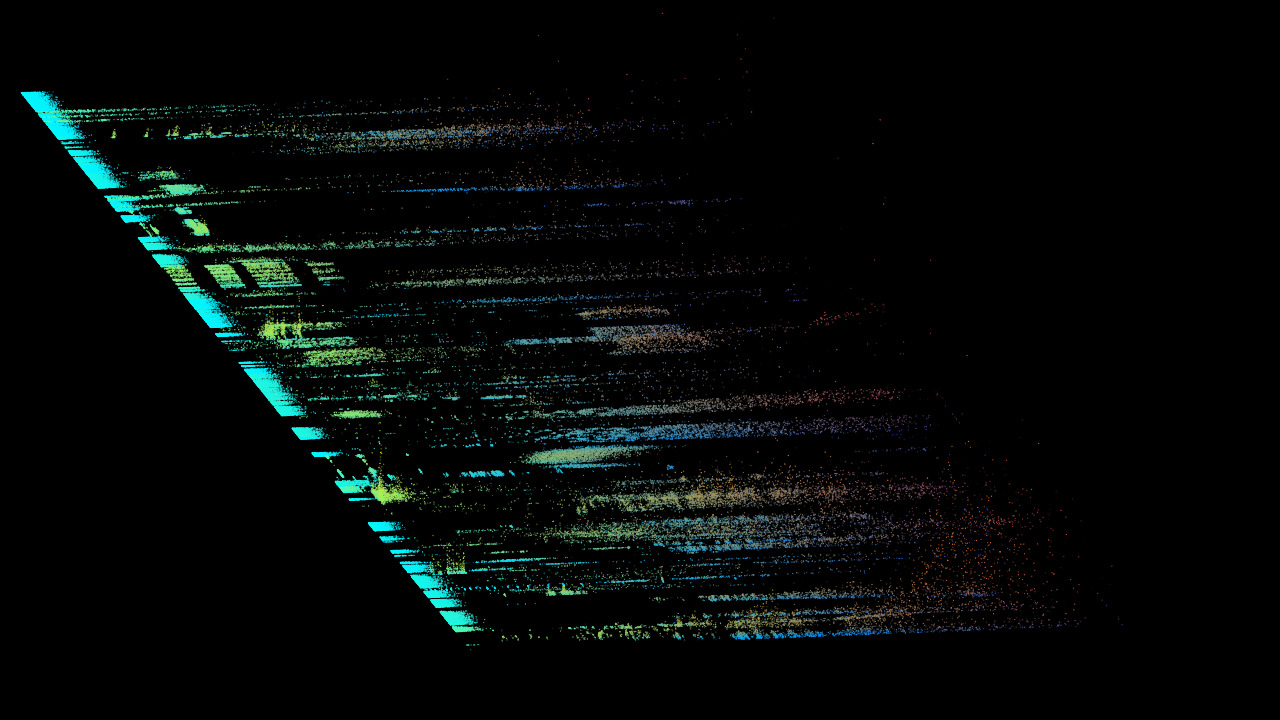
\includegraphics[width=\linewidth]{preset-50-14.jpg}%\par
\end{multicols}
\begin{multicols}{2}
    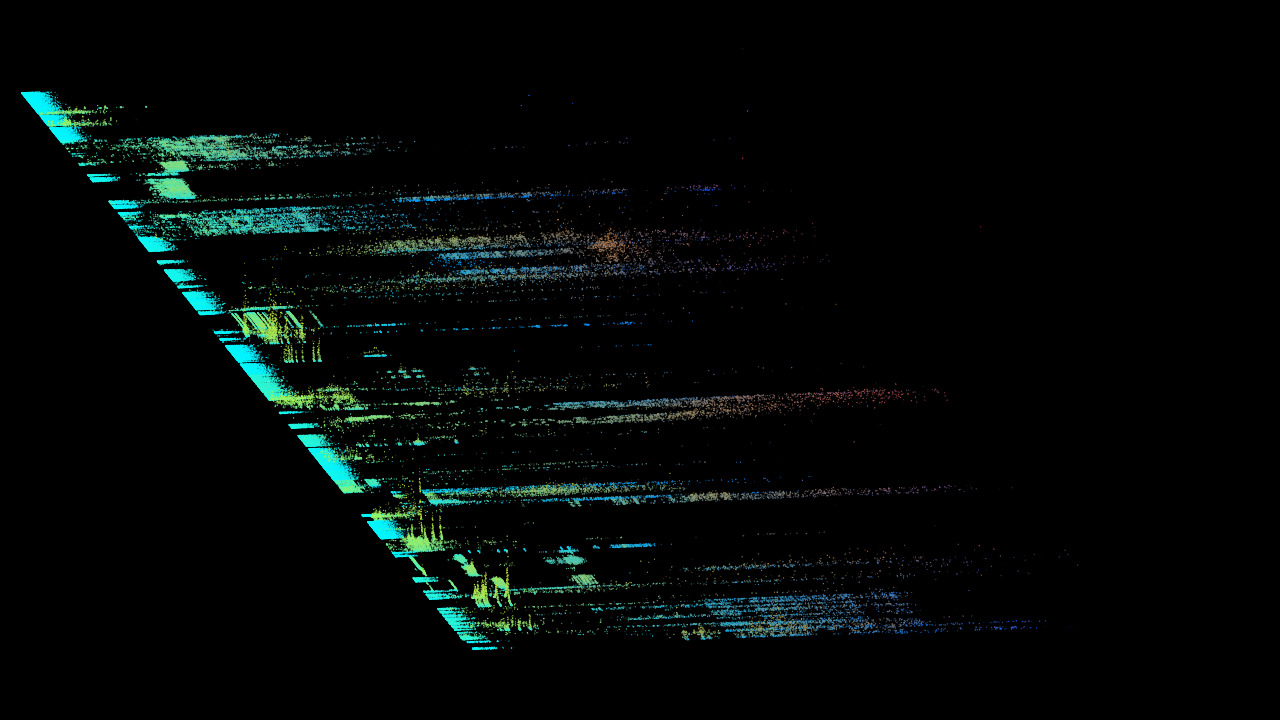
\includegraphics[width=\linewidth]{preset-50-5.jpg}%\par 
    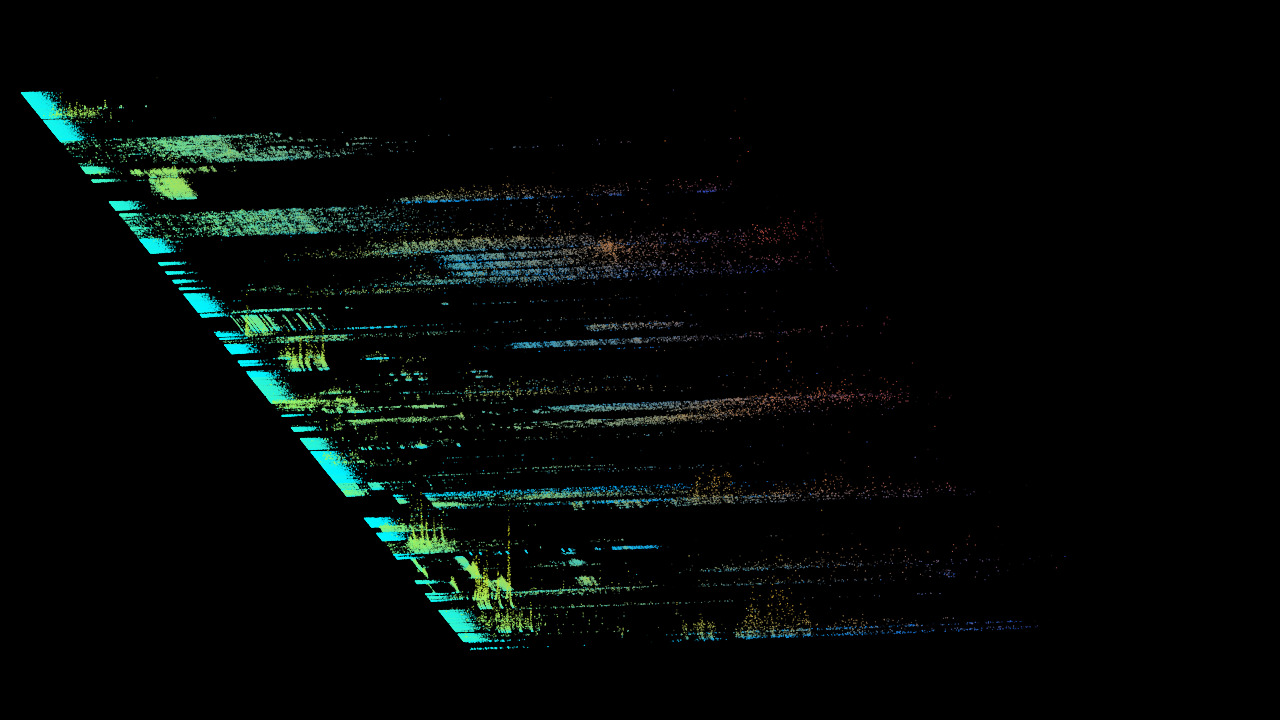
\includegraphics[width=\linewidth]{preset-50-6.jpg}%\par 
\end{multicols}

\caption{Tracks 5-6 (below) and 13-14 (above).}
\end{figure*}



Despite the disadvantages delineated above, I considered [sigmund\~{}] to be a very accurate tool for the purposes of this paper. The output of [sigmund\~{}] when in peaks mode, is as follows:

\begin{itemize}
\item frequency (Hz)
\item amplitude (RMS)
\item cosine component (real value)
\item sine component (imaginary value).
\item lo malo es que justamente a esa altura, cuando casi nadie ha aprendido a remontar la piedrita hasta el Cielo,
\item se acaba de golpe la infancia 
\item y se cae en las novelas, 
\item en la angustia al divino cohete, 
\item en la especulaci\'{o}n de otro Cielo al que tambi\'{e}n hay que aprender a llegar. 
\end{itemize}




As in every visualization, there are several elements at stake in bringing information into display in a meaningful manner. There are also the limitations of the tool for visualizing in itself. I chose to stay within Pd and load a library called ``Graphical Interface for Multimedia'', or Gem. Using Pd as a programming language --amongst other things--, Gem is in its core a C++ wrapper for OpenGL.\footnote{https://puredata.info/downloads/gem/documentation/manual/pub/danks1997realtime.pdf} Several people have contributed over the years in making Gem what it is now.\footnote{From Gem's welcome message: Mark Danks (original version), Chris Clepper, Cyrille Henry, IOhannes m zmoelnig, Guenter Geiger, Daniel Heckenberg, James Tittle, Hans-Christoph Stein{\dots} et al.} From within this rather large library, I only used one key object called [gemvertexbuffer]\footnote{Authors: Cyrille Henry, Antoine Villeret, jprtzk and IOhannes m zmoelnig} for the actual plotting of the spectra. This object allows the rendering of a Vertex Buffer Object (VBO),\footnote{https://www.khronos.org/opengl/wiki/Vertex\_Specification} which is essentially an array of data stored in the Graphical Processing Unit (GPU). The object accepts several arrays for the different attributes such VBO can hold. In this case, I only provided a position array and a color array. 


\begin{figure*}

\begin{multicols}{2}
    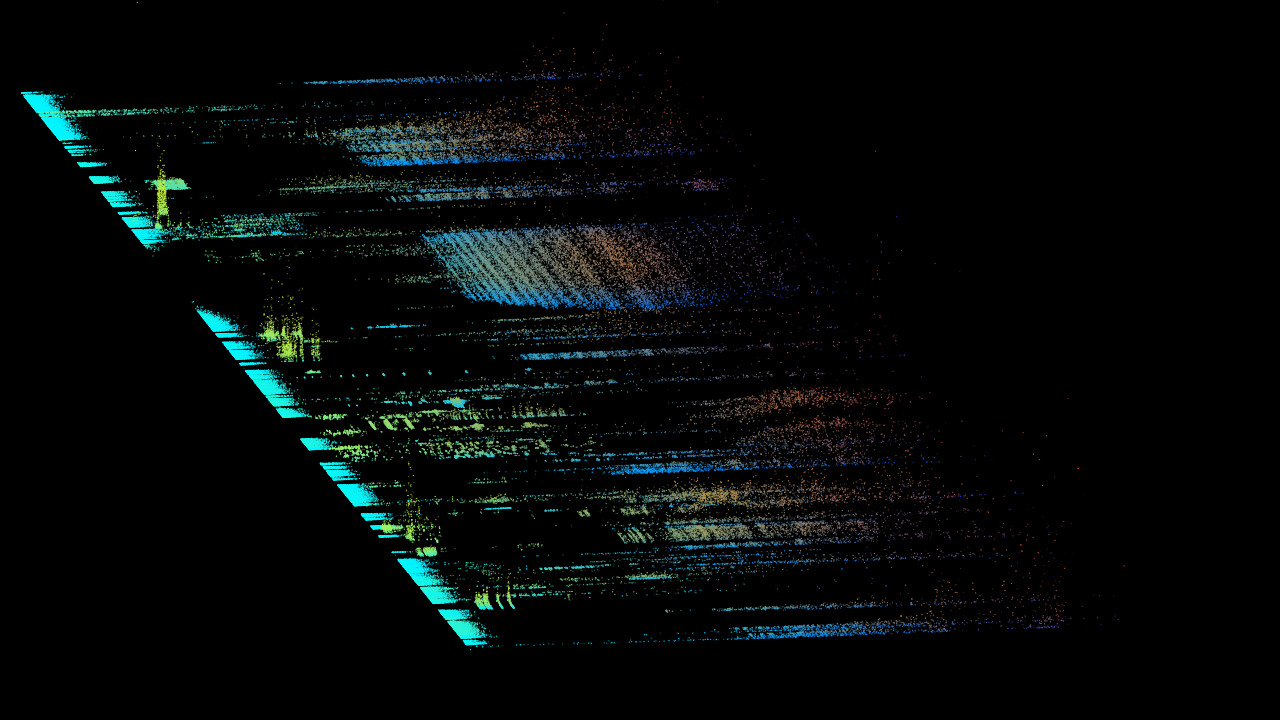
\includegraphics[width=\linewidth]{preset-50-15.jpg}%\par
    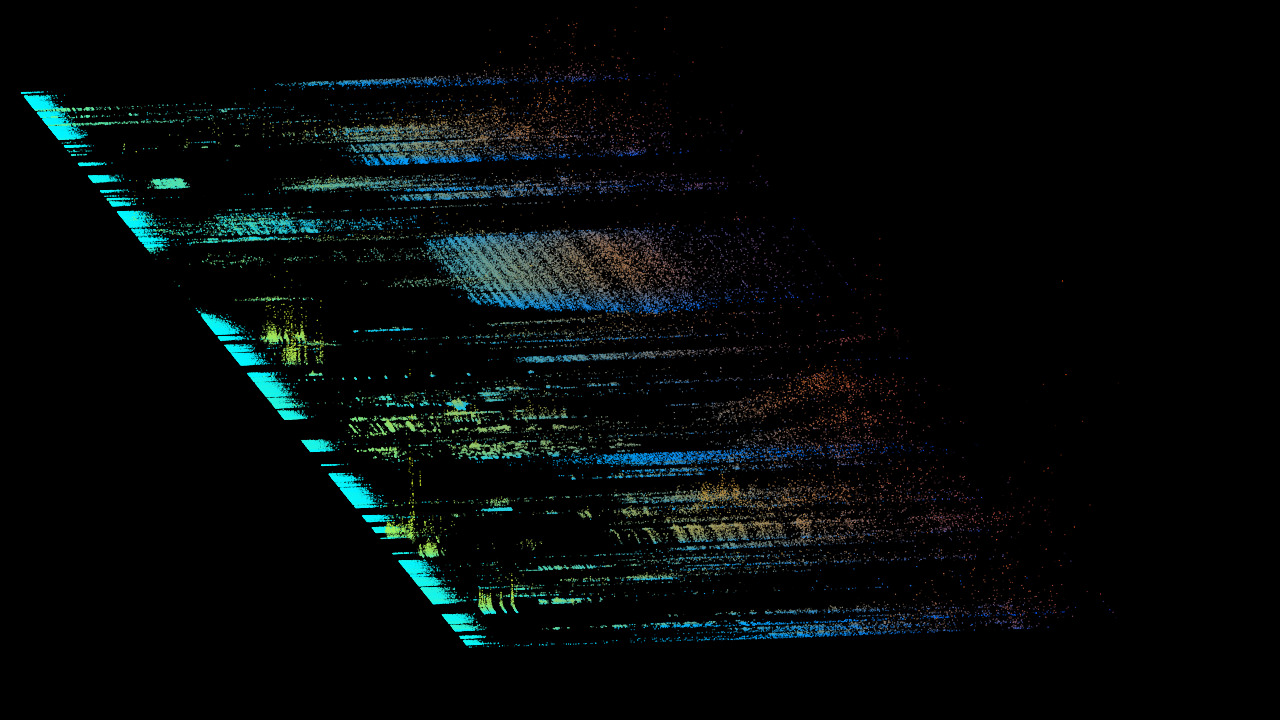
\includegraphics[width=\linewidth]{preset-50-16.jpg}%\par
\end{multicols}
\begin{multicols}{2}
    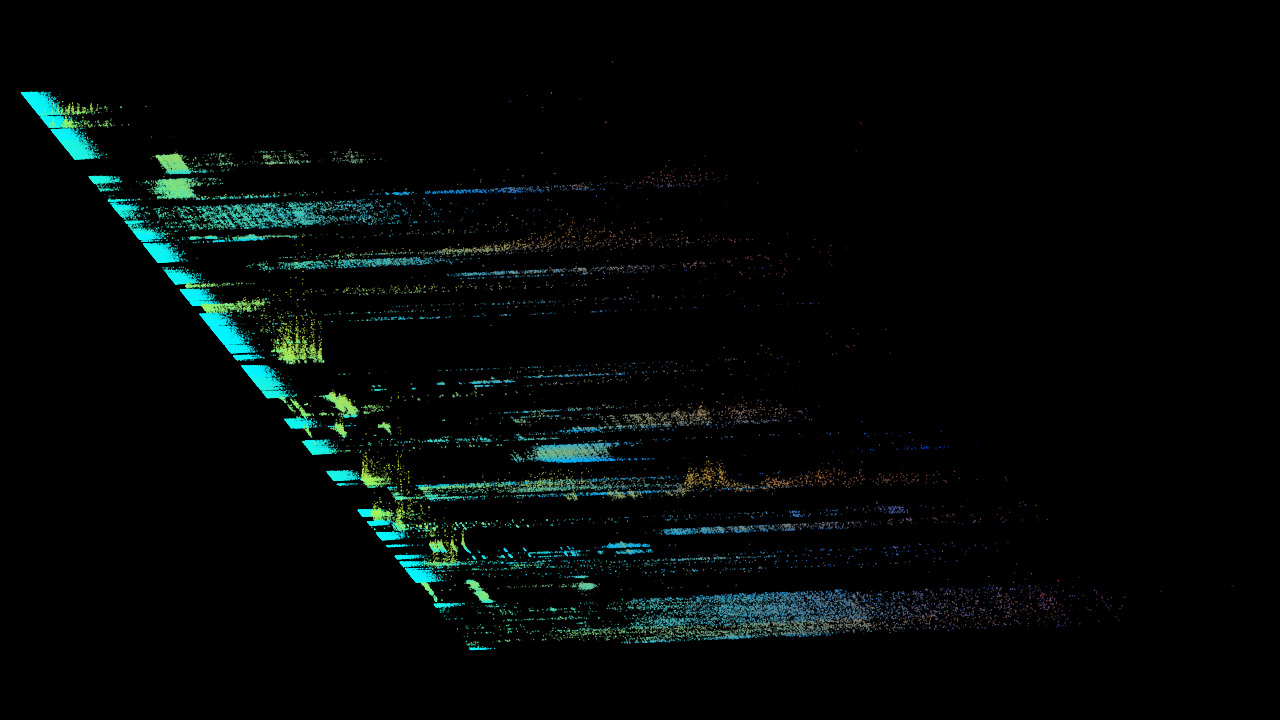
\includegraphics[width=\linewidth]{preset-50-7.jpg}%\par 
    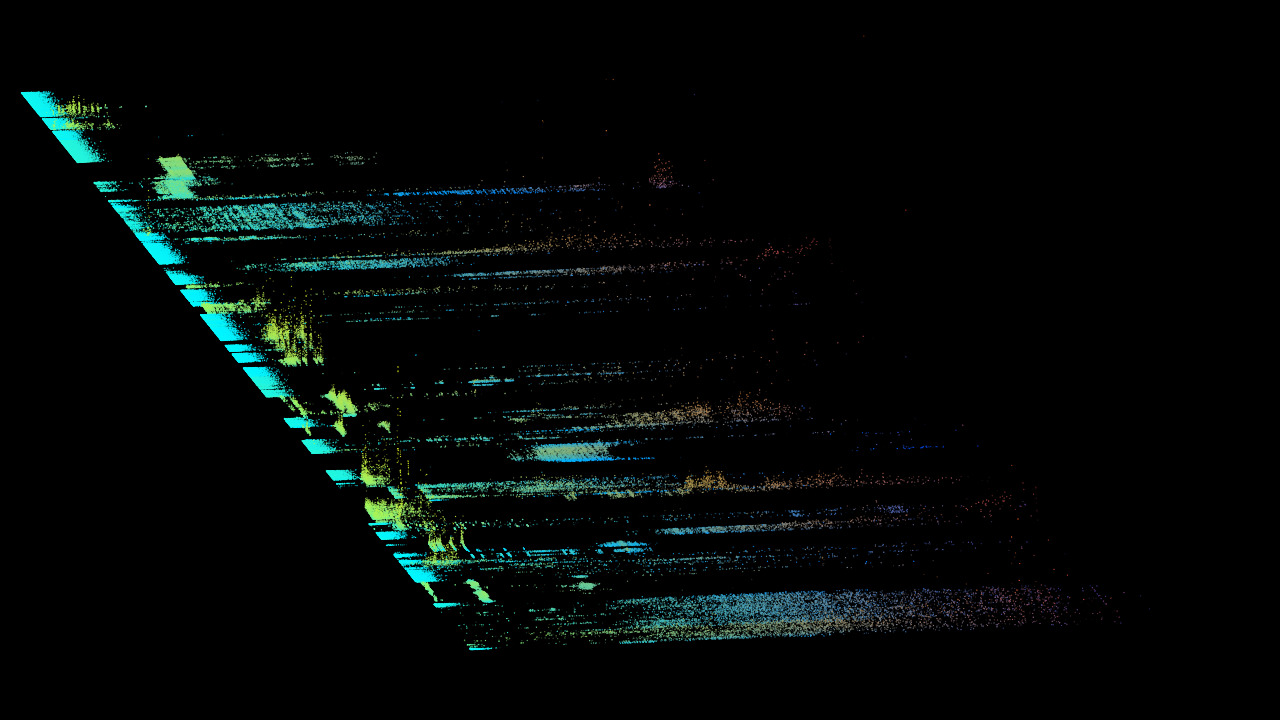
\includegraphics[width=\linewidth]{preset-50-8.jpg}%\par 
\end{multicols}
\caption{Tracks 7-8 (below) and 15-16 (above). The color of the points displays Amplitude and Frequency in a different manner: Red and Blue act as a continuum of amplitude (Red being an amplitude of 1 and Blue an amplitude of 0) and Green shows Frequency (a higher frequency means more Green). The Alpha channel shows Phase information: the closer to $\pi$ the more visible, and the closer to -$\pi$, the more transparent it is.}
\end{figure*}


In order to plot the spectrum in time, the position array is built with  $x=\log (\mathit{frequency})$,  $y=\mathit{amplitude}$, and  $z=\mathit{time}$. Once these attributes are set, the VBO can be further manipulated (scaled, \ rotated, translated, etc), so some manipulations were made for the image to be rendered in a functional way (for example, in the center of the screen). Since the Z-axis holds time information, time-variation within the plot needs to be read from what is farthest to what is closests. Furthermore, since the amplitude is shown as a function of the frequency, the frequency space is rendered in an inverse way on the X-axis, the highest frequencies going towards the left and the lower ones towards the right. Finally, since amplitude is on the Y-axis, and since the rendered peaks appear as individual points, it is difficult to grasp at first sight where each point belongs to in a static image.\footnote{If one has control of the position of the VBO and the scale, then its three-dimensionality is grasped immediately.} 

%
%
%\begin{center}
%\begin{figure*}
%
\includegraphics[width=3in]{foryoungears-img002.png}
%\caption{Spectrum of visible light.}
%\end{figure*}
%\end{center}
%
\newpage
The color information is set as an Red, Green, Blue and Alpha (RGBA) normalized color array, and it is built as follows: $R=\mathit{rmstodb}(\mathit{amplitude})$;  $G=\log (\mathit{frequency})$;  $B=1-R$;  $A=\arctan (\Re ,\Im )$.\footnote{All of these values were normalized between 0-1.} This means several things. First of all, the transparency of the points (Alpha value) introduces the angle (or phase) of the peak.\footnote{The impact of phase in timbre seems to be more prominent for frequencies below 200 Hz (Park, 2004). In these visualizations, however, transparency can only be seen by enlarging the time axis and the point sizes, and the linear mapping of phase to the alpha channel was done without consideration to the above mentioned research.} 
 The rest of the values depend on the position information. Like the X-axis, the Green value is the logarithm (for visual scaling purposes) of the frequency, so if the point is towards the left of the screen it will have more Green than towards the left. The same happens to the Red value: like the Y-axis, more amplitude means more Red value. Finally, since color synthesis in the screen is additive, whenever these three value (RGB) increase altogether, they tend towards white, and if they decrease, they tend towards black. This is why the Blue value is the inverse of the Red, which means that less amplitude (and less Red) will provide more Blue value. Drawing a perceptual analogy with the color spectrum of visible light (figure 1), Green or Yellow can constitute the high frequency bands (the most visible, towards the center), and Blue or Red the low frequency bands (the least visible, towards the edges).

\paragraph{Cyan Line}
There are a few elements to consider when describing the Cyan line that runs accross the entire visualization, occupying a band from the highest frequecy analyzed with [sigmund\~{}] (here 16 kHz) to about 7 kHz. At first, I thought it to be simply high-frequency noise resulting from the windowing of the analysis. However, it has been noted the possibility of this being peak analysis of what is called `dither', a small amount of noise added by multitrack audio softwares to compensate for quantization errors from bit resolution reduction.\footnote{ After conducting several tests, it seems that there is indeed a band of pseudorandom numbers that constitute an inaudible noise in the range above 7 kHz in all of the tracks. I kindly thank Dr. Jaime Oliver for this suggestion. See https://en.wikipedia.org/wiki/Dither\#Digital\_audio} Nevertherless, despite the fact that it emerges out of an analytical misfortune, what this line reveals is the void in each track and it is evidence of her treatment of silence and orchestration throughtout the piece. Whenever the Cyan line is present it is when dithering is present, that is, when there is silence in the track. While within a stereo image, the Cyan lines draw almost parallel patterns (revealing once again the paired construction), when comparing between stereo images, they reveal very different patterns: visual evidence of the spatial distribution of energy. In my opinion, it is this abundance of \emph{cyan} within each track what allows the overall pristine quality of the sound which is why I dedicated so much visual presence to this line. 
\begin{figure*}
\begin{center}
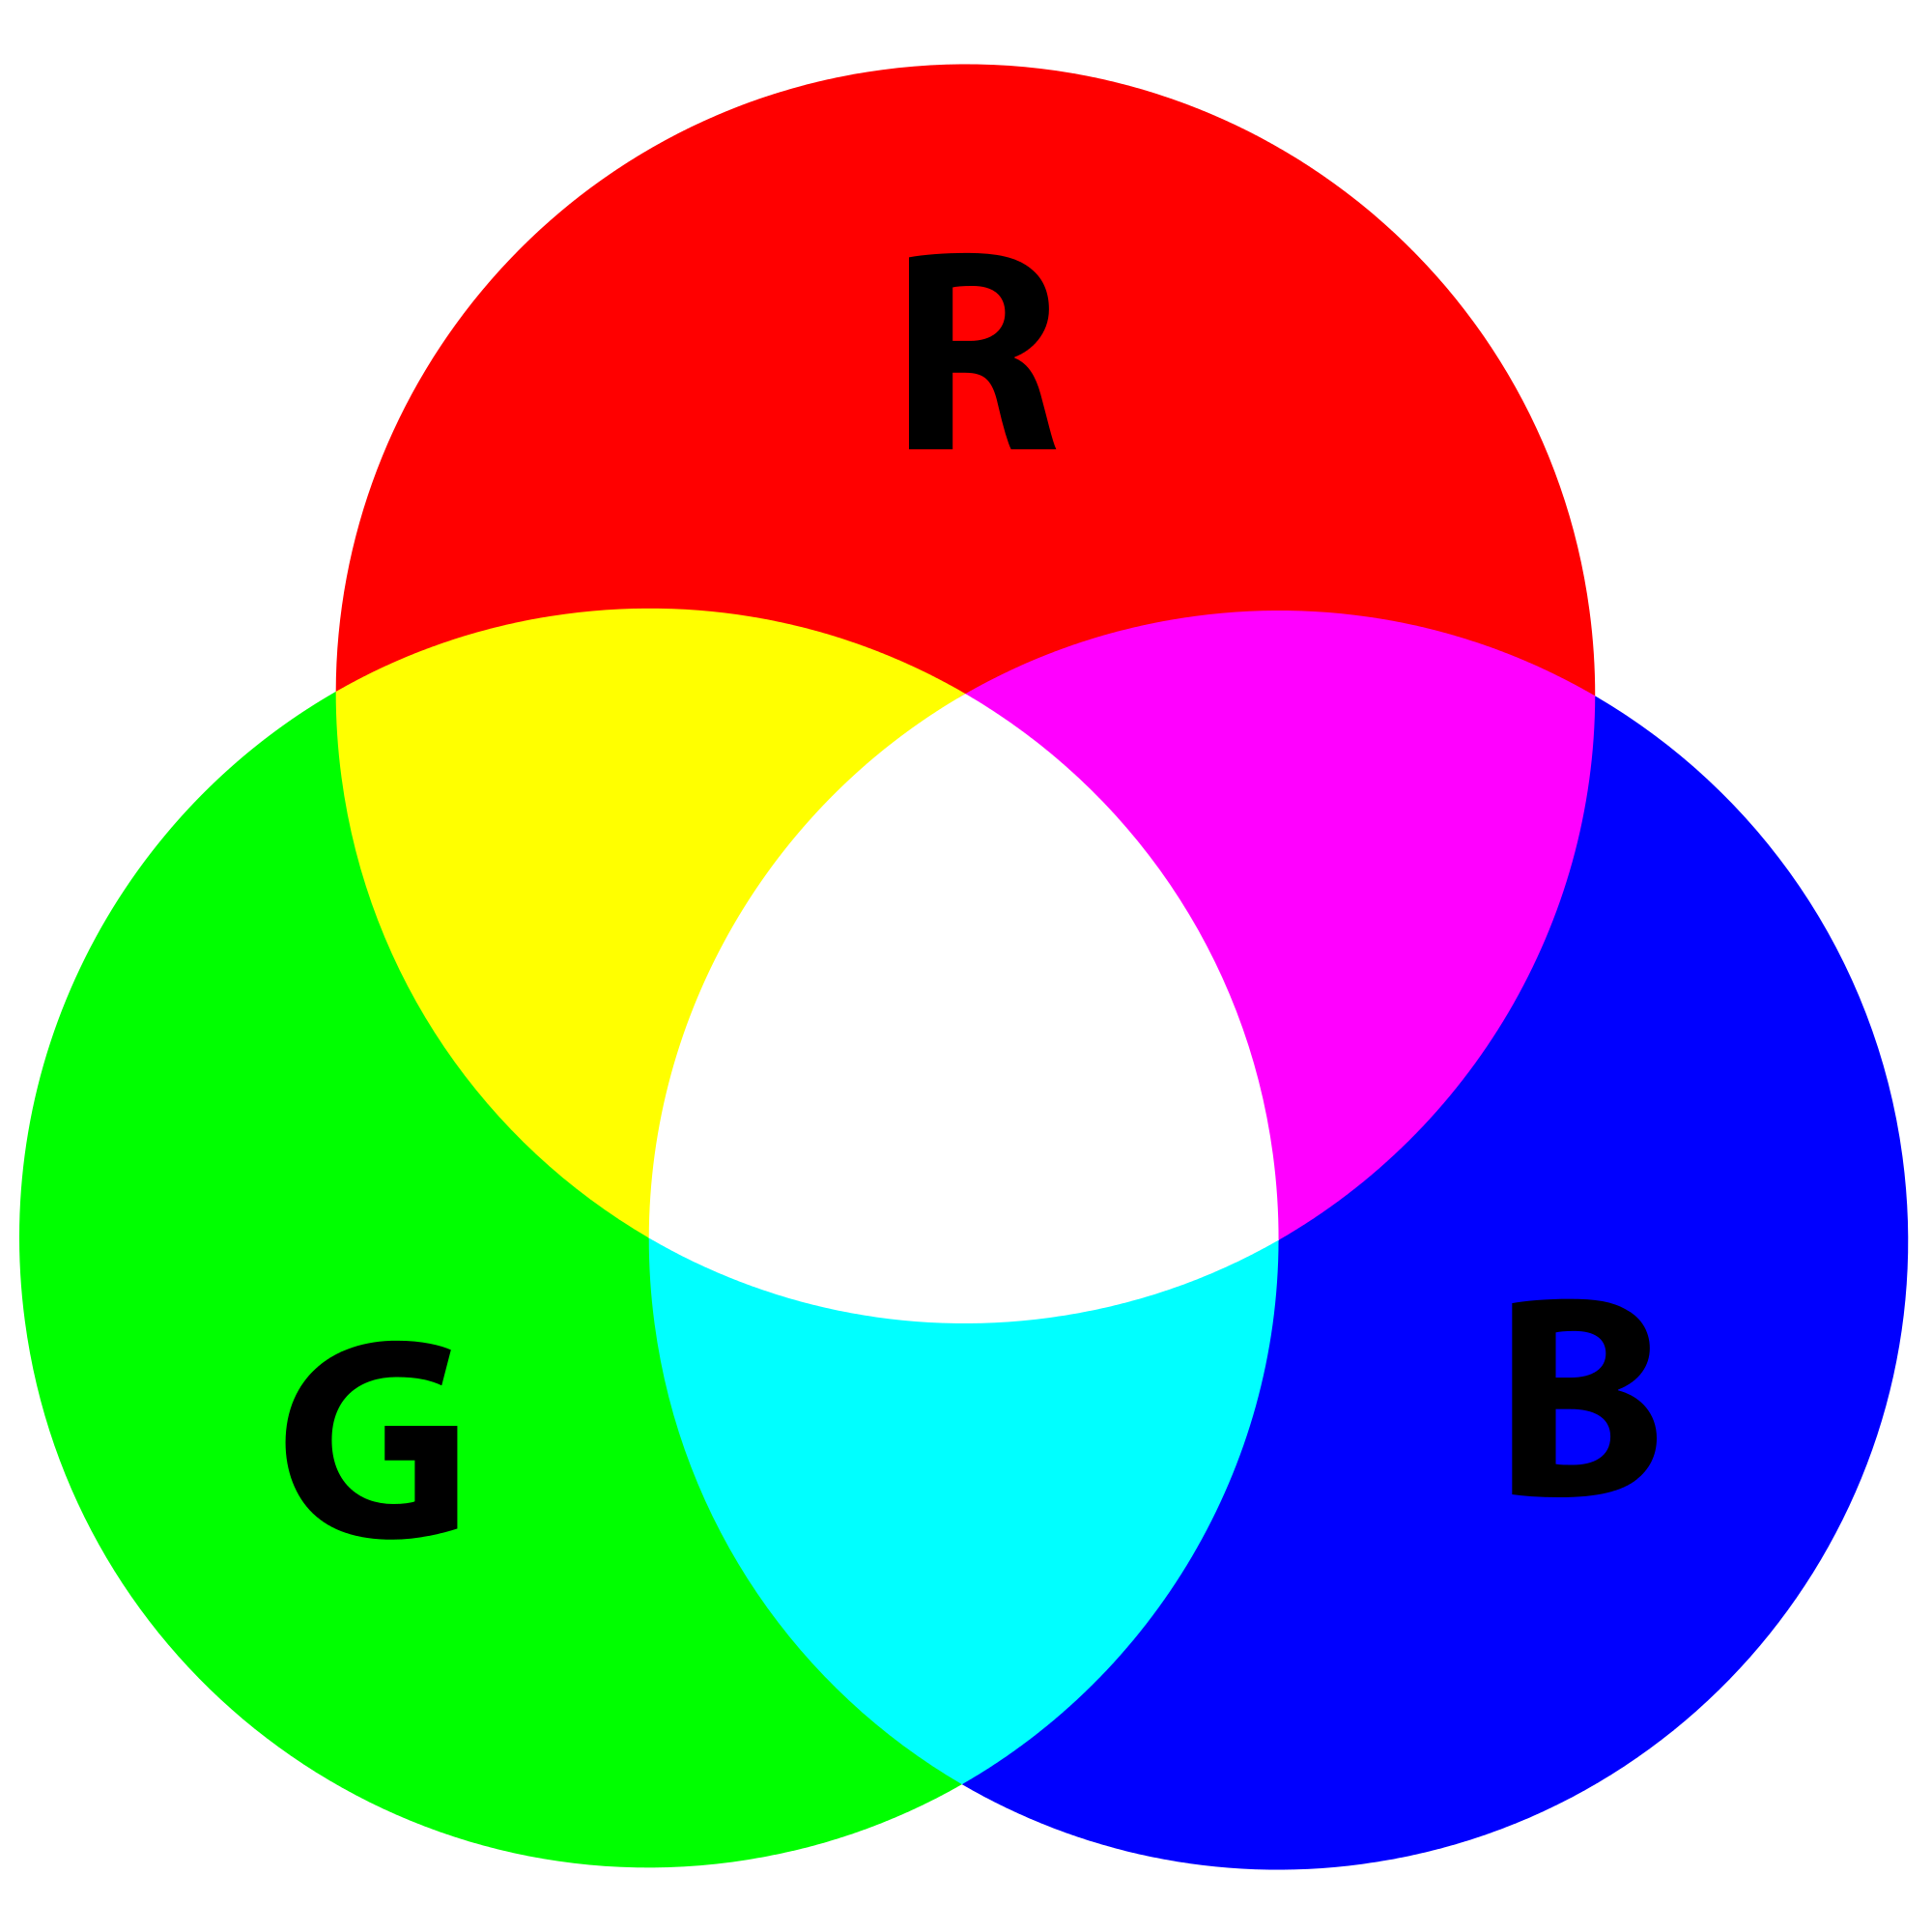
\includegraphics[width=1.5161in,height=1.5161in]{foryoungears-img004.png}
 \caption{Color synthesis chart: In general, from these visualizations, quiet sounds will have Blue tonality, loud sounds will be Red, and high-pitched sounds will have high frequency content, so if a sound is high and loud it will be Yellow, if it's low and quiet it will be around Magenta and if it is high and quiet, Cyan.}
\end{center}
\end{figure*}




\newpage



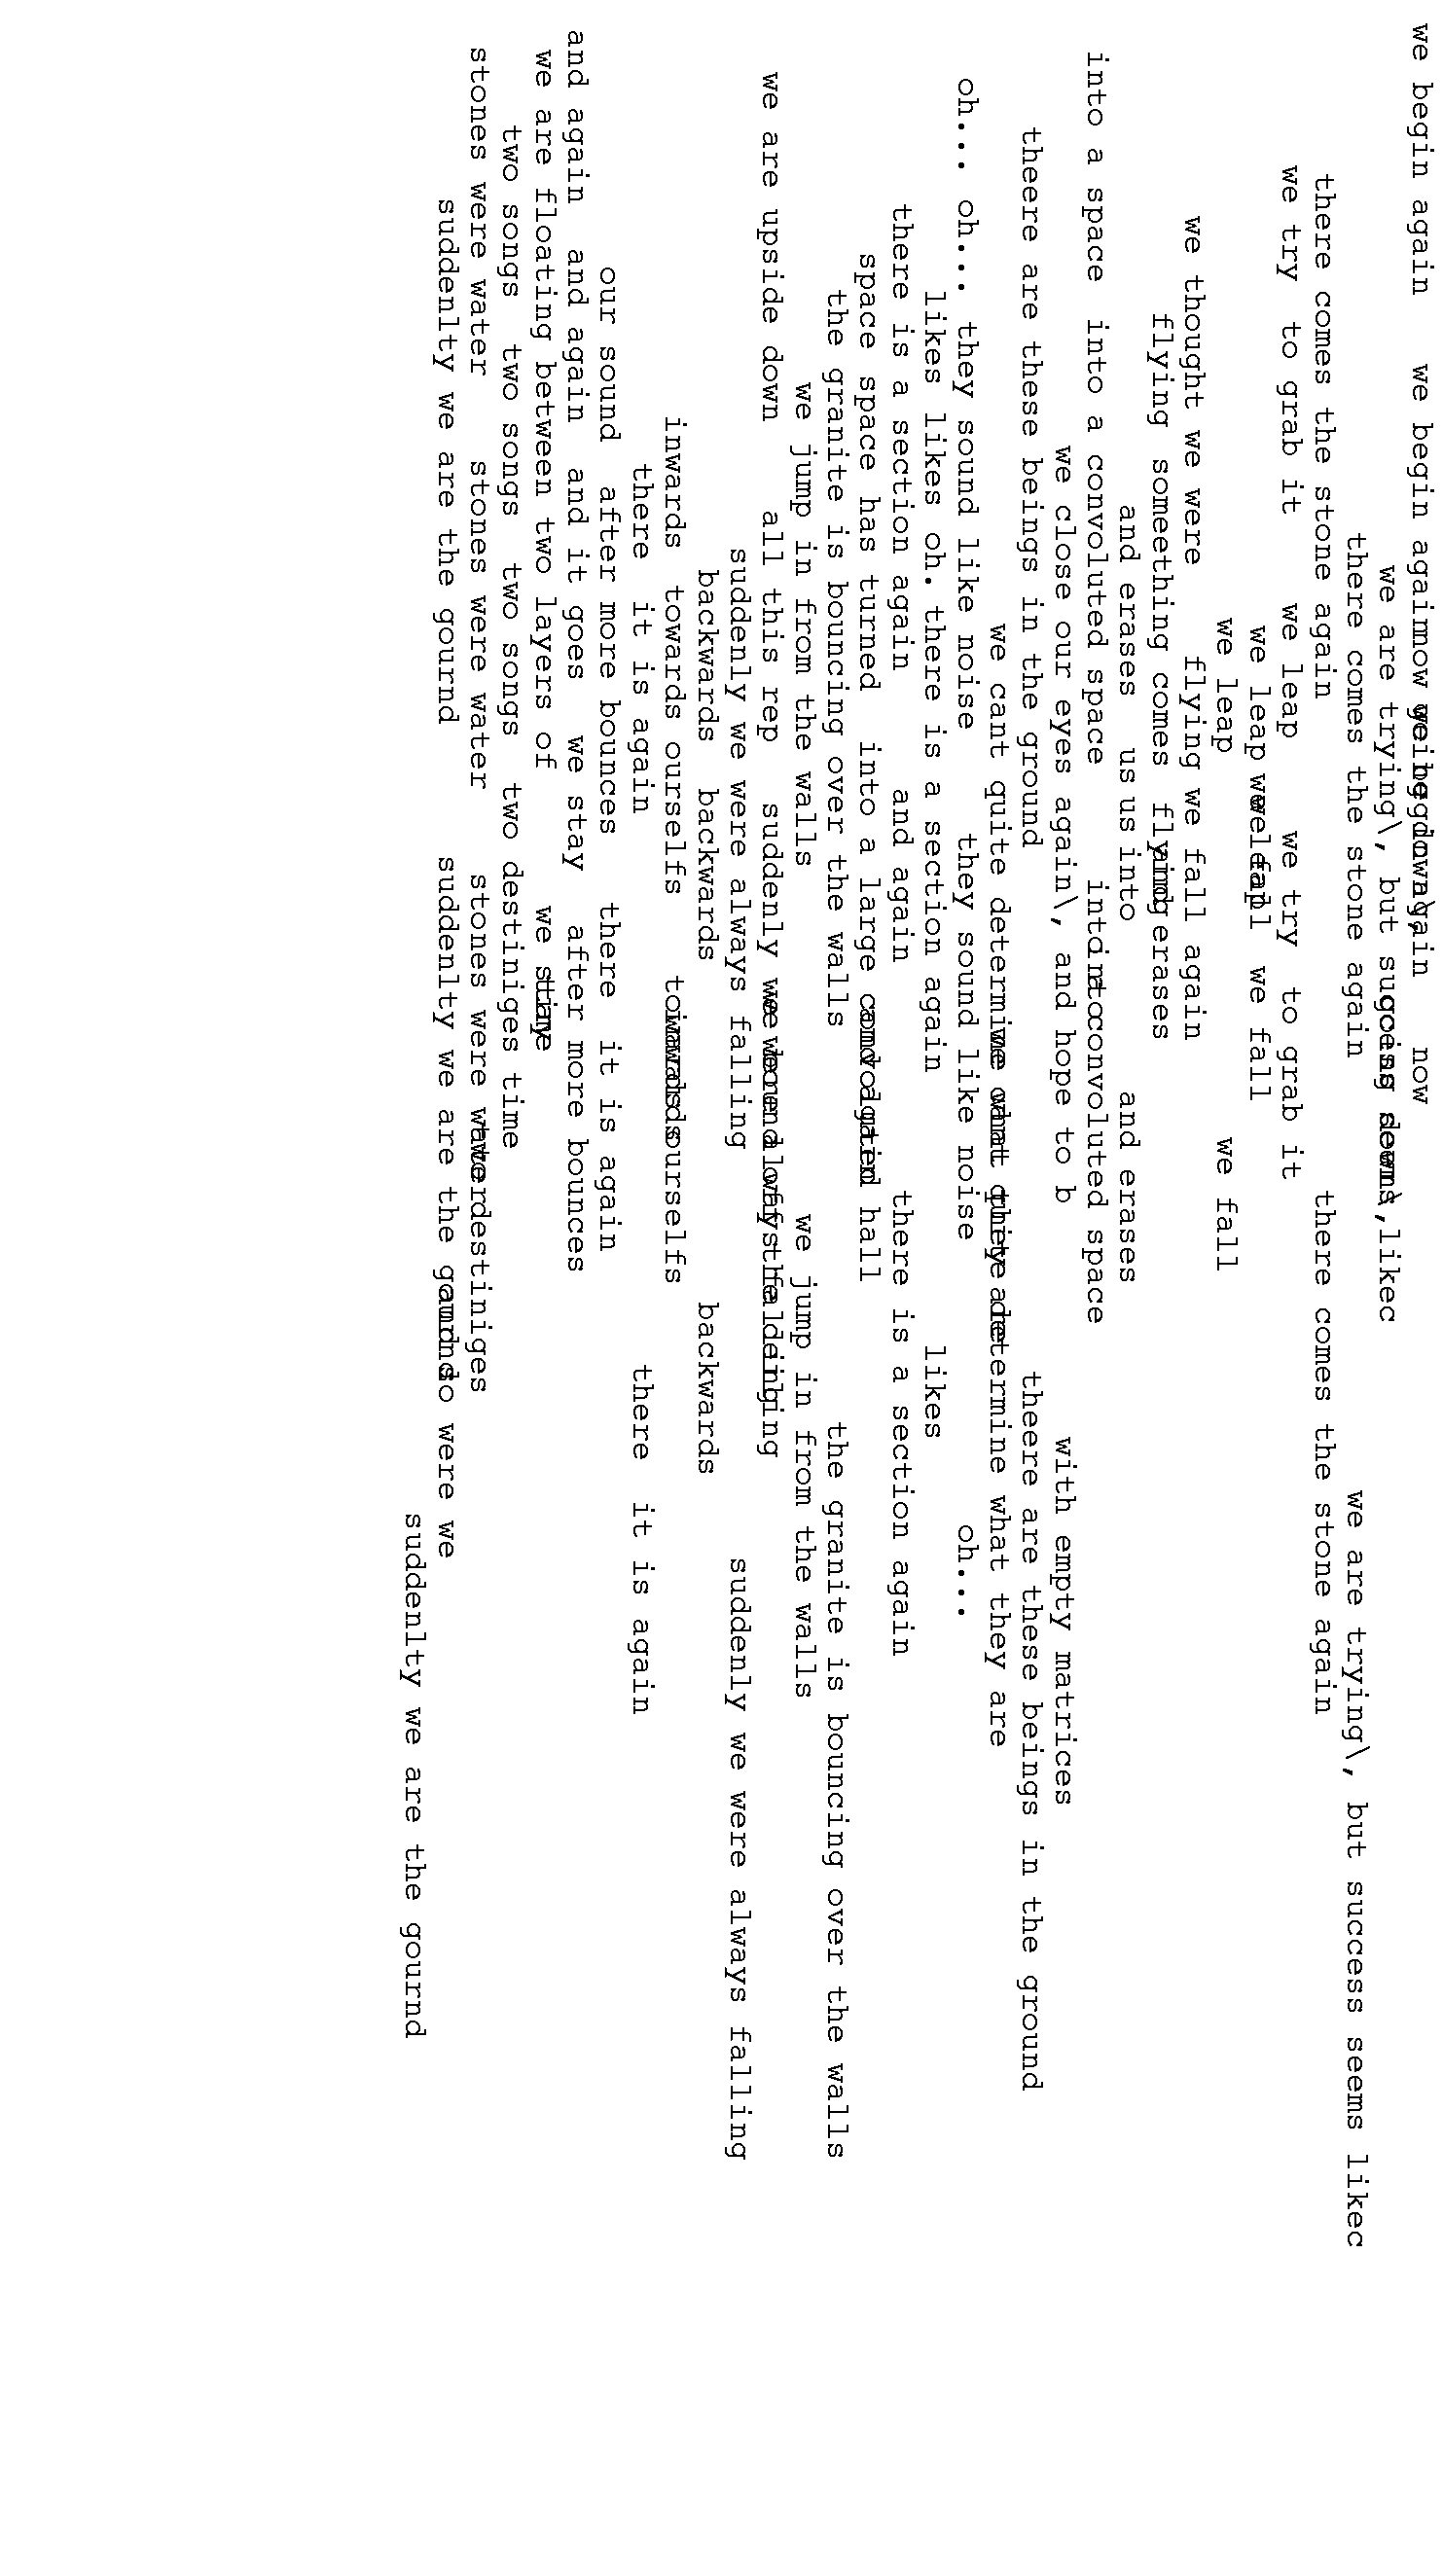
\includepdf[pages={1}]{../pdf/sub-6.pdf}

\begin{center}
\begin{figure*}

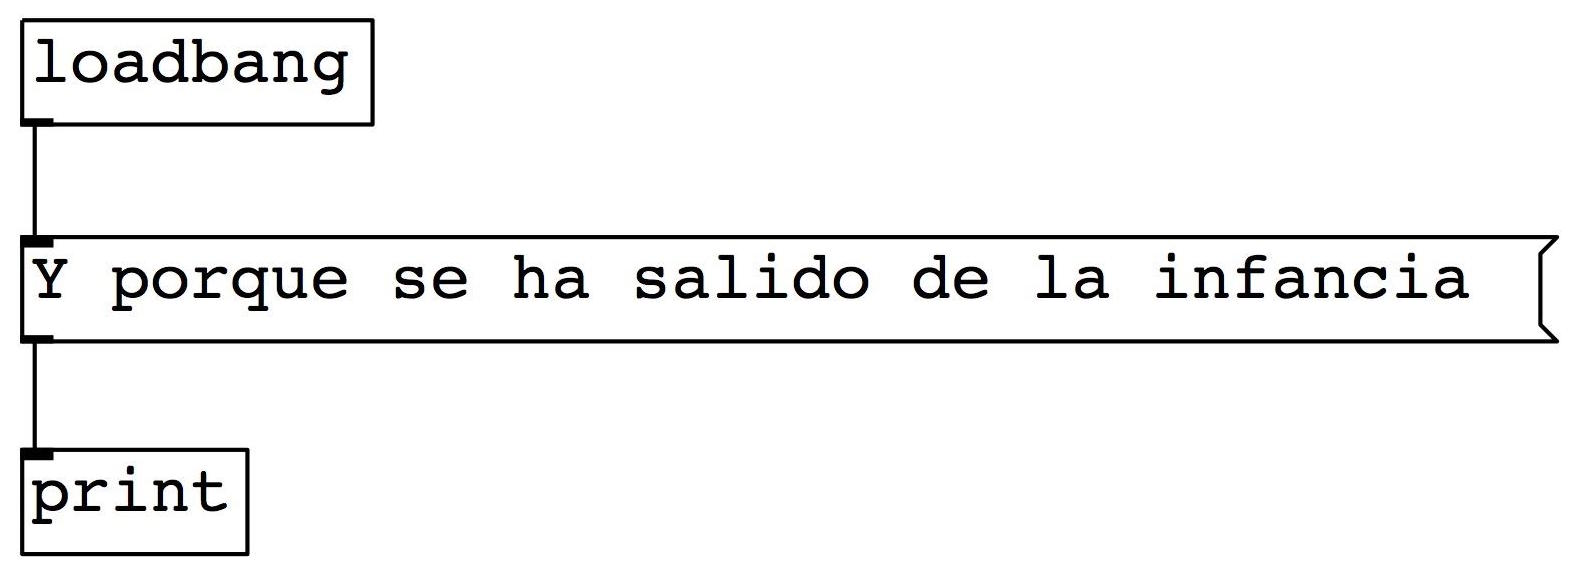
\includegraphics[width=3in]{foryoungears-img003.jpg}
\caption{print: Y porque se ha salido de la infancia}
\end{figure*}
\end{center}
In trying to visualize \textit{Marelle}, considering the fact that tracks needed to be assigned in pairs, my hypothesis was that it was in fact composed as spatial layers of stereo images, that is, from eight stereo images between speakers on both sides of the room arriving at an expanded stereo field. What is interesting about these plots, however, is that they show a different treatment of the spatial image when the four stereo pairs of the bottom are compared with the four elevated stereo pairs. What first comes to view is that there are elements present in one and absent in the other. But, this is not as simple as it reads. These uncorresponded elements not only appear distributed in different moments in time, they appear in different sections of the spectrum. What is more, they reveal a precise use of negative space, in the sense that what is around the sculpted shapes is just as important as the shapes itself. It is important to note that this is not just negative visual space in my visualization, it is an inherently sonic and thoroughly composed phenomenon.


\bigskip
\begin{flushright}
(Je n'oublierai pas le temps des c\'{e}rises, patale\'{o} Emmanu\`{e}le en el suelo) 
\end{flushright}


\bigskip

As an example of this distribution, I'd like to focus on the middle section of tracks 15 and 16. The greatest salience in figure 4 is in tracks 15-16 (above): around the center of the image (the middle of the piece) there appears a very expressive bridge-like shape covering a rather large time frame and a large section of the mid-low frequency band. When compared to the rest of the tracks, while there certainly are some similar shapes in that same moment in tracks 5,6,9 and 10, one can see that the closest shape resembling this salience is in track 12 (figure 2, above-right). What is more, while this shape is taking place, one sees in 1,2,3,4,11,13 and 14, similar shapes in the higher frequencies, but with less amplitude. Finally, the two remaining tracks (7-8) show a very different behavior altogether: set of higher frequency bands are displayed (in yellow). Ultimately, what this particularly complex distribution of energy shows is a multidimensional sculpting of an aural image.

I would also like at this point to perform some sort of criticism. In the last image of this response, I place one of my favorite sounds in this piece, what I call a `bird' sound: a loud and very high frequency sound sweeping irregularly from 10 to 14 kHz.q This sound which appears on track 15 is replicated with some very minimal decorrelation (14 milliseconds) in track 16 (i.e., from left to right in this stereo image). Although this is a well known technique for stereo (Kendall, 1995; Vaggione, 2001), and it is evident that its effectiveness and beauty is out of the question, I wonder if this decorrelation had been not with in its adjacent pair, but within the speakers no.15 and 9, or between 15 and 9 and 3, or between $1$ and $N-1$ peakers. What I mean to suggest here is not that there is a fault in the piece, merely that however efective it is, there is some degree of loss in translating one technique (stereo imaging) from one medium (stereo) into another (16 speaker array with elevation).\footnote{This analogy with language is also one of the reasons why there is a text in spanish traversing this response.}

\bigskip


\begin{flushright}
\textit{My greatest pleasure when listening to this piece came through the rhythmic treatment. She managed to build conglomerates of gestures on top of each other, flying from one side of the room to the other, from one band of the spectrum to the other; reflecting, rotating and intertwining bright shapes, all  engaging in contrapunctal phrases, evoking simultaneously elaborate medieval poliphonies and the sound of sand.}
\end{flushright}
\newpage

This distribution of \emph{spectromorphologies} --to borrow Denis Smalley's famous concept-- prove that \textit{Marelle} ``seeks to embrace the full spectral potential of the wide-open sound world'' (Smalley, 1997). In other words, her exploration of spectral space, as displayed in these visualizations, can be understood as a gesture towards the limits of perception. When Dr. Justel populates with energy the extremes of the frequency space, she sets forth two different aesthetic agents. The agency of these bands, however, is given by the composer in the shapes she builds within these spectral areas: the hand-crafted use of amplitude. Each one has a singular treatment that can only be achieved by a very tight feedback with the resulting sound. It is this extremely detailed treatment of Form within the distinct spectral regions what gives expressiveness and an idea of unity between the two extremes, which in turn means cohesion and operational coherence. Going one step further, Dr. Justel's craft resides not only in her elaborate technical skills, but also in her ability to project this union of the extremes as a metaphor of life. The player of Hopscotch = Marelle = Rayuela --as Julio Cort\'{a}zar's description reads-- starts from \emph{Earth} and plays through space with a stone, hopping unpredictably until she reaches a \emph{Sky}.

\bigskip

\begin{figure*}
\begin{multicols}{2}
    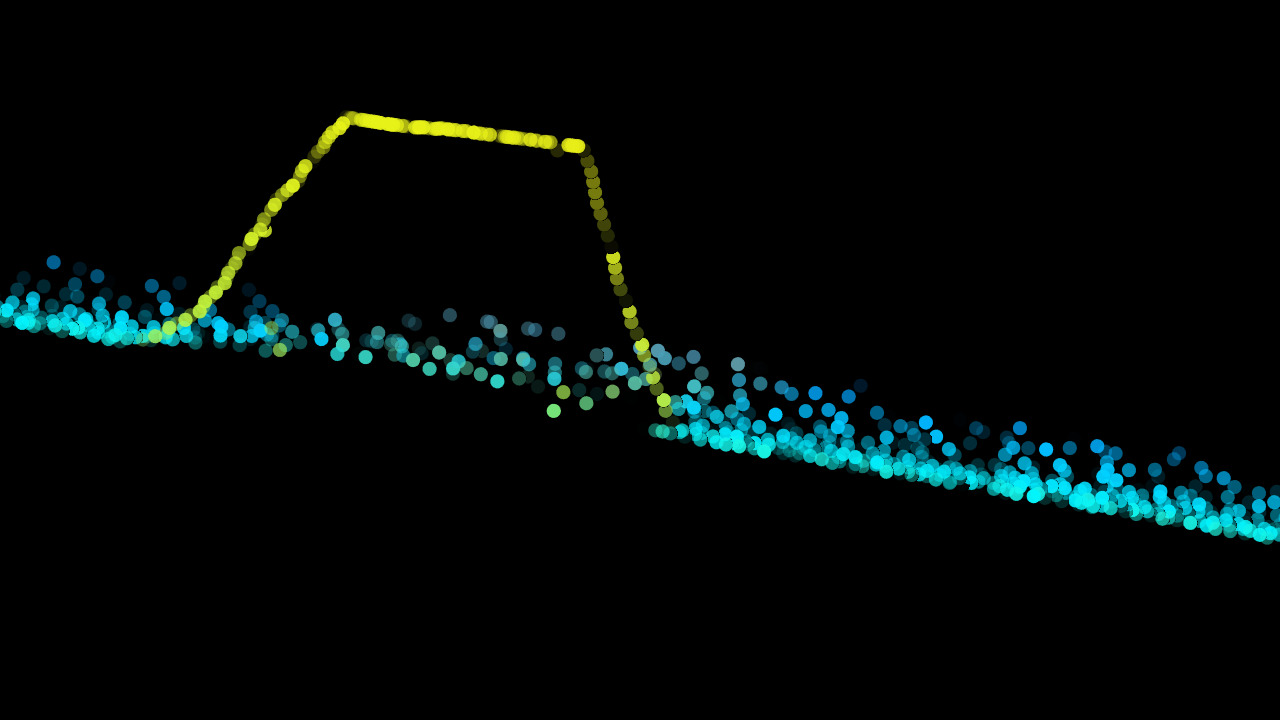
\includegraphics[width=\linewidth]{preset-31-elsa-7100000.jpg}%\par
    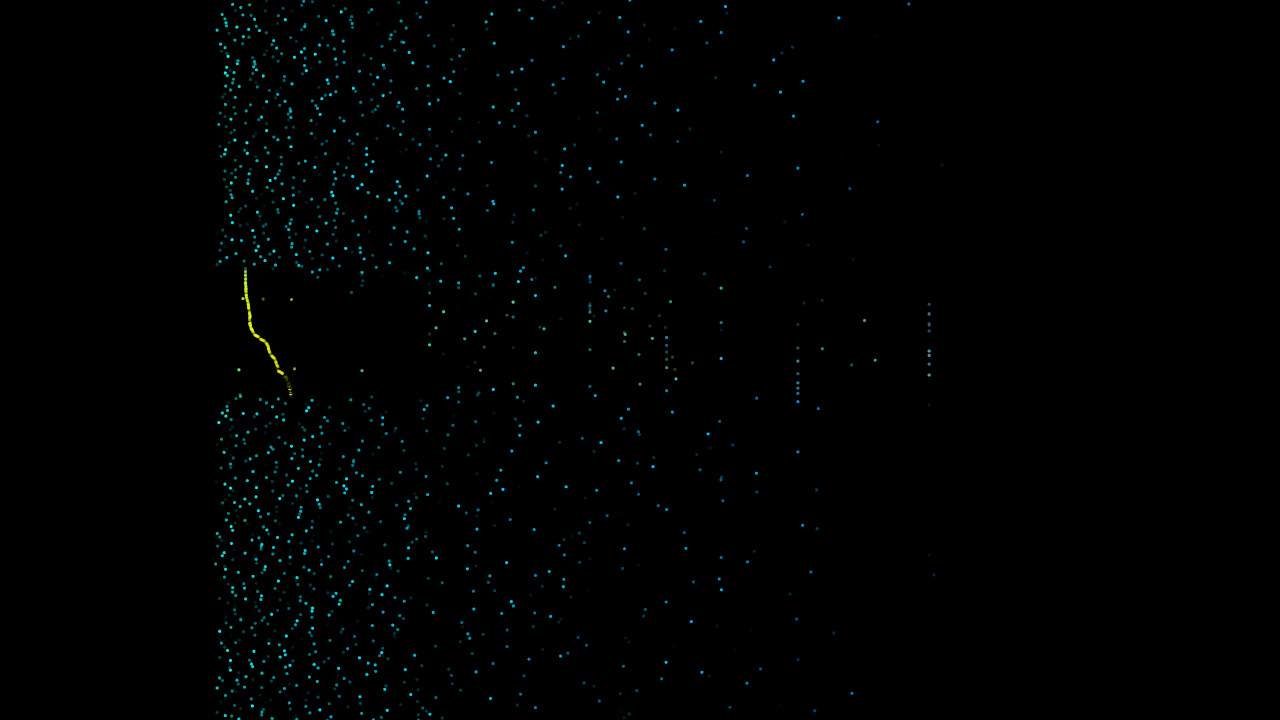
\includegraphics[width=\linewidth]{preset-56-elsa-7300000.jpg}%\par
\end{multicols}
\caption{Track 15:2'48'' capture of 48000 samples (above). Bird sound.}
\end{figure*}


\bigskip

\textit{
At points, one can hear some source material almost unfiltered but in most cases the source is a residual image leading to intimate evocations of water and close-mic techniques. }


\bigskip

se olvida que para llegar al Cielo se necesitan, como ingredientes, una piedrita y la punta de un zapato.''\footnote{Chapter 36 (Cort\'{a}zar,1963)}



\bigskip
\bigskip

I first heard Elsa Justel's \textit{Marelle} at the New York City Electroacoustic Music Festival NYCEMF, in June 2017. It was performed at the Experimental Music Theatre of the Abrons Art Center. After the concert I approached her and congratulated her, and she said: ``this is for young ears''.
\bigskip
\bigskip
\paragraph{Coda}
\textit{
Dr. Hoffmann: ``Finally : for young ears.  Say more: what did Elsa mean? do you agree?''\footnote{Taken of an email from Dr. Elizabeth Hoffman}}
\bigskip

During that very quick moment after her performance, I took her words to mean that given the amount of activity in the high register, and the abundance of spatial motion, \emph{Marelle} would appeal, in her opinion, to the younger generation of today. At one point I considered Presbycusis\footnote{https://en.wikipedia.org/wiki/Presbycusis} as an age delimiter (the bird, for example, might not be heard by ``old'' ears). However, I resist to think this way. I believe that in her mind she is addressing youth, not as a sector of society, but as an aesthetic agent. Youth becomes the driving force in her exploration of sound and space: with these ears, every sound is a new world; every movement, a new way of being; every moment, a constant \emph{now}. Within the spectral playground she created, I would even suggest the following: The playfulness with which she approaches space throughout the piece is as intense as the seriousnes with which a kid would attempt to reach the sky during recess.

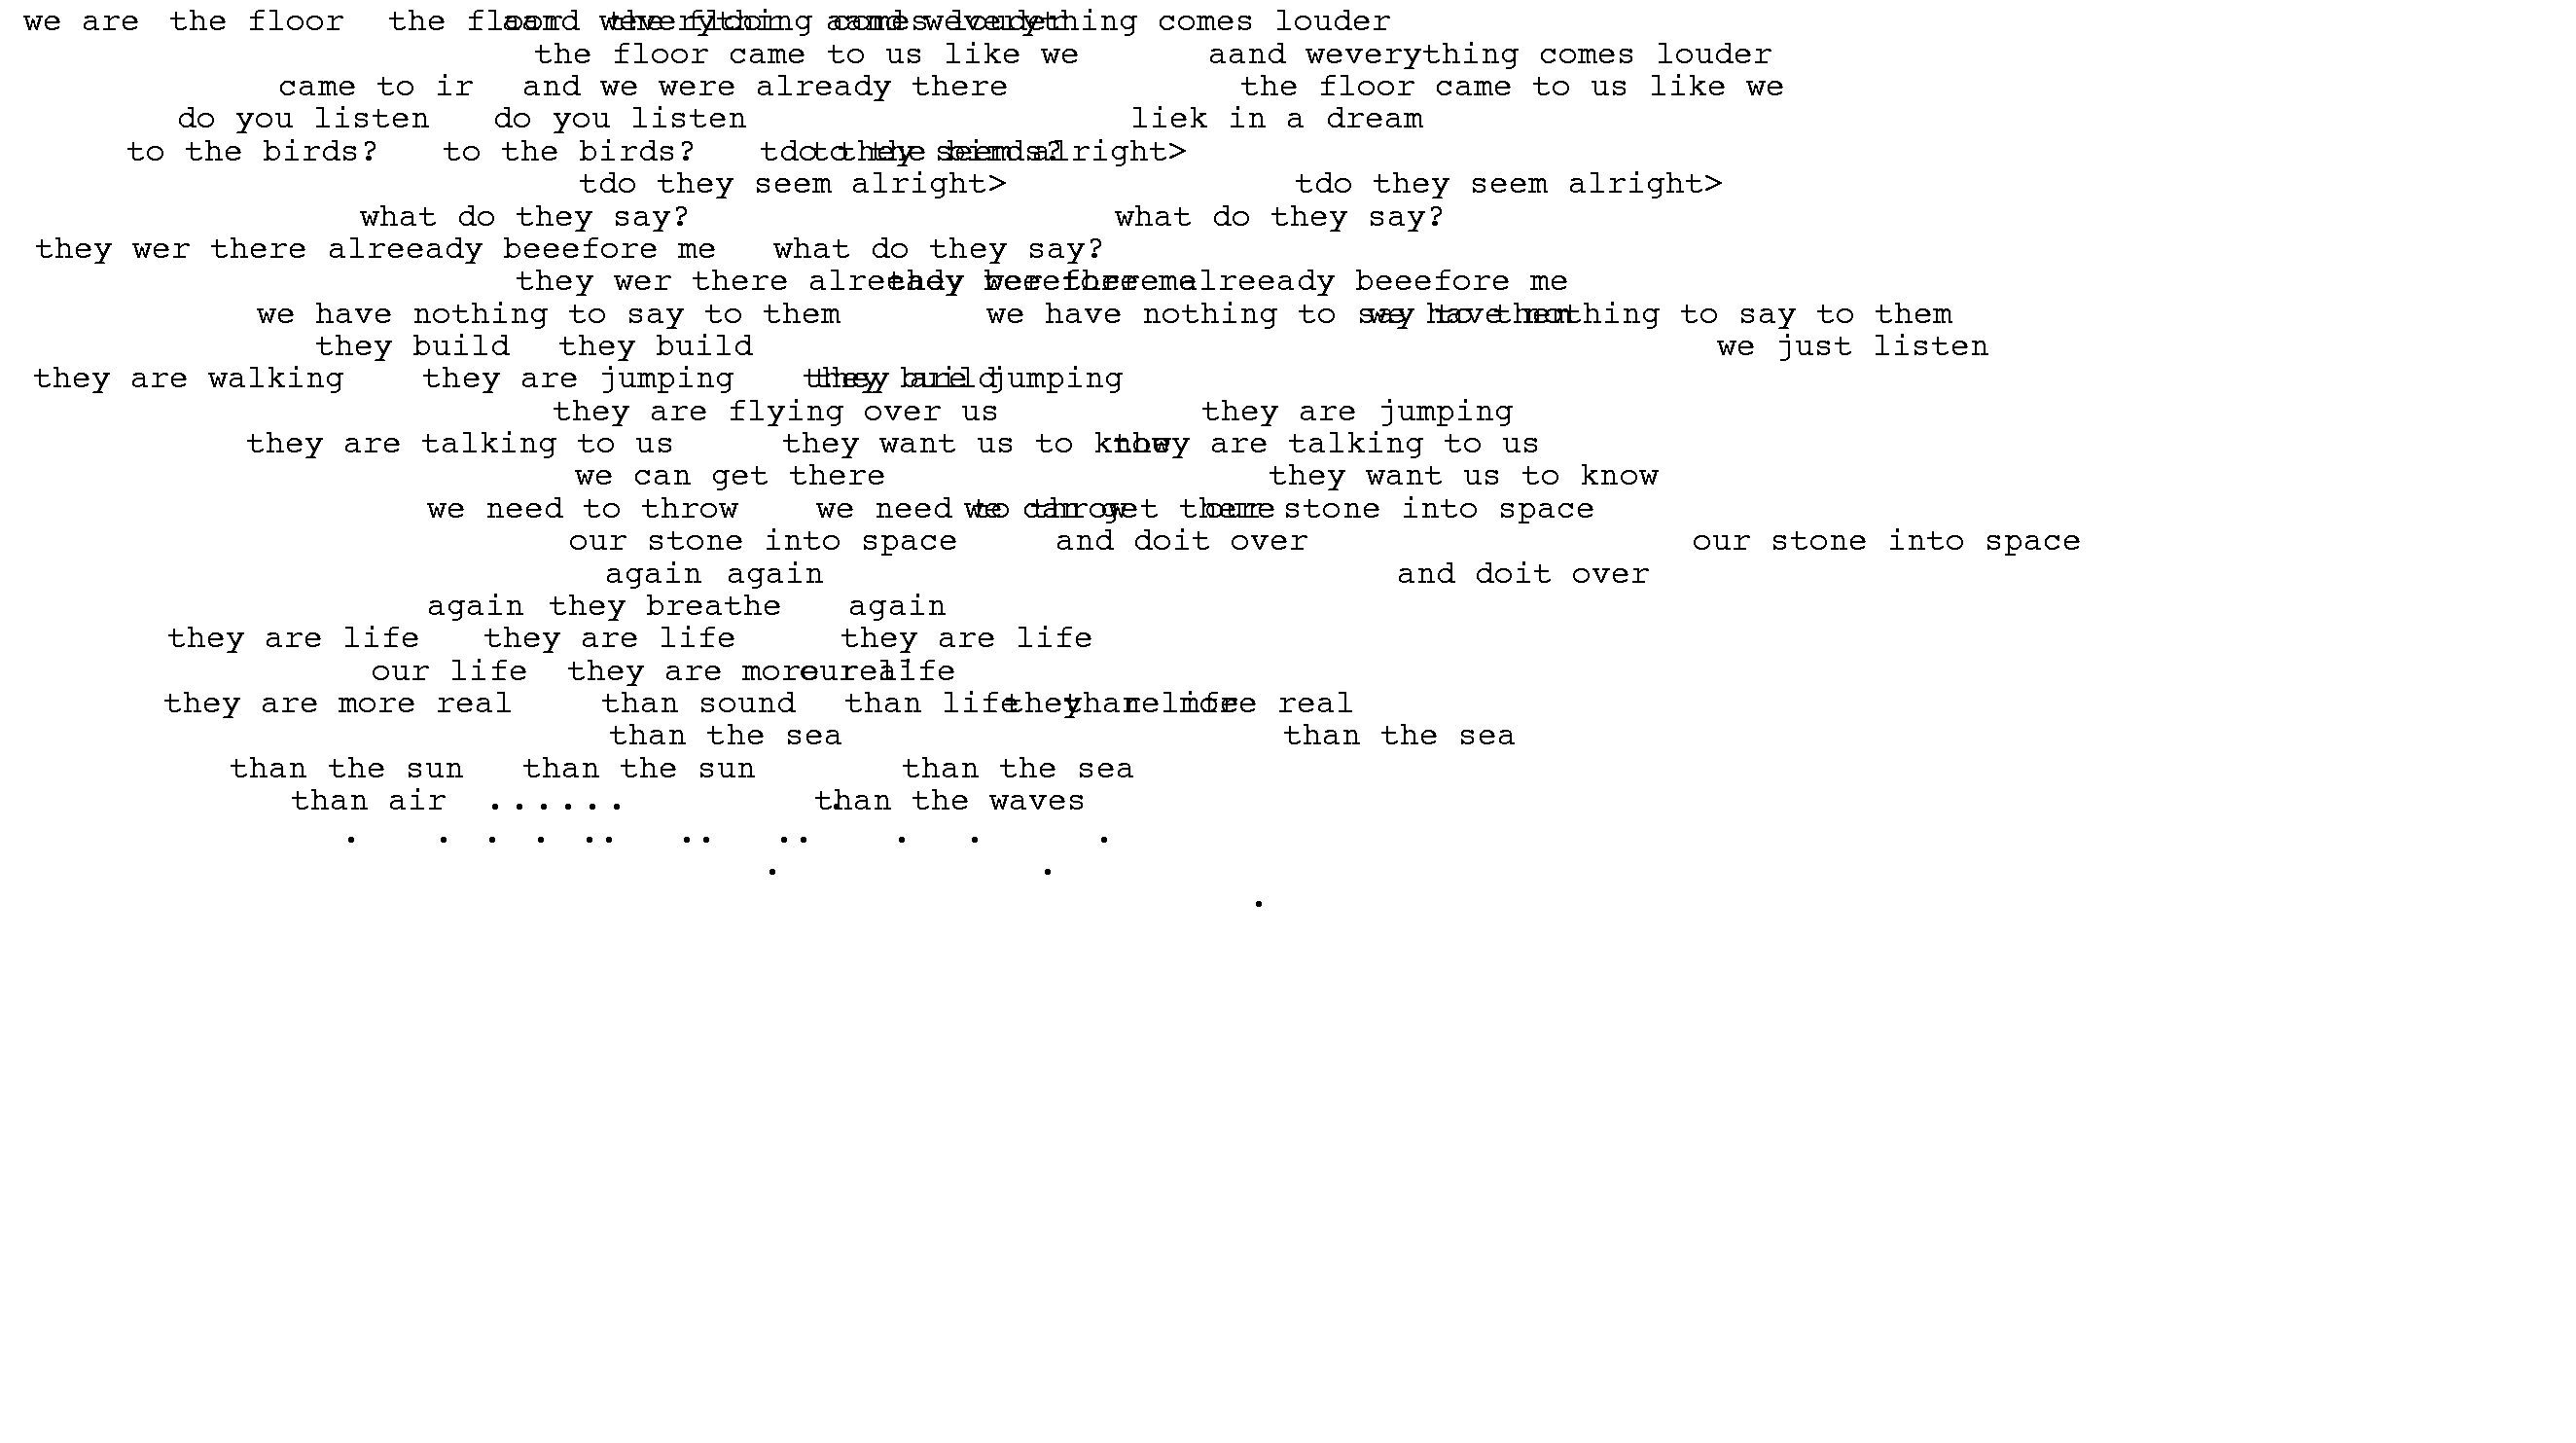
\includepdf[pages={1}]{../pdf/sub-7.pdf}


\end{document}
